% !TEX TS-program = XeLaTeX
% use the following command:
% all document files must be coded in UTF-8
\documentclass[english]{textolivre}
% build HTML with: make4ht -e build.lua -c textolivre.cfg -x -u article "fn-in,svg,pic-align"

\journalname{Texto Livre}
\thevolume{15}
%\thenumber{1} % old template
\theyear{2022}
\receiveddate{\DTMdisplaydate{2022}{4}{25}{-1}} % YYYY MM DD
\accepteddate{\DTMdisplaydate{2022}{7}{6}{-1}}
\publisheddate{\DTMdisplaydate{2022}{9}{20}{-1}}
\corrauthor{André de Oliveira Matumoto}
\articledoi{10.35699/1983-3652.2022.39398}
%\articleid{NNNN} % if the article ID is not the last 5 numbers of its DOI, provide it using \articleid{} commmand 
% list of available sesscions in the journal: articles, dossier, reports, essays, reviews, interviews, editorial
\articlesessionname{articles}
\runningauthor{Matumoto and Gonçalves-Segundo} 
%\editorname{Leonardo Araújo} % old template
\sectioneditorname{Daniervelin Pereira}
\layouteditorname{Leonado Araújo}

\title{Towards a social-semiotic approach to visual analysis of two-dimensional games: a toolkit}
\othertitle{Análise visual de jogos bidimensionais: uma abordagem por meio da semiótica social}
% if there is a third language title, add here:
%\othertitle{Artikelvorlage zur Einreichung beim Texto Livre Journal}

\author[1]{André de Oliveira Matumoto \orcid{0000-0003-3544-3576} \thanks{Email: \href{mailto:andrematumoto@usp.br}{andrematumoto@usp.br}}}
\author[1]{Paulo Roberto Gonçalves-Segundo \orcid{0000-0002-5592-8098} \thanks{Email: \href{mailto:paulosegundo@usp.br}{paulosegundo@usp.br}}}
\affil[1]{Universidade de São Paulo, Faculdade de Filosofia, Letras e Ciências Humanas, Departamento de Letras Clássicas e Vernáculas, SP Brasil.}

\addbibresource{article.bib}
% use biber instead of bibtex
% $ biber article

% used to create dummy text for the template file
\definecolor{dark-gray}{gray}{0.35} % color used to display dummy texts
\usepackage{lipsum}
\SetLipsumParListSurrounders{\colorlet{oldcolor}{.}\color{dark-gray}}{\color{oldcolor}}

% used here only to provide the XeLaTeX and BibTeX logos
\usepackage{hologo}

% if you use multirows in a table, include the multirow package
\usepackage{multirow}

% provides sidewaysfigure environment
\usepackage{rotating}

% CUSTOM EPIGRAPH - BEGIN 
%%% https://tex.stackexchange.com/questions/193178/specific-epigraph-style
\usepackage{epigraph}
\renewcommand\textflush{flushright}
\makeatletter
\newlength\epitextskip
\pretocmd{\@epitext}{\em}{}{}
\apptocmd{\@epitext}{\em}{}{}
\patchcmd{\epigraph}{\@epitext{#1}\\}{\@epitext{#1}\\[\epitextskip]}{}{}
\makeatother
\setlength\epigraphrule{0pt}
\setlength\epitextskip{0.5ex}
\setlength\epigraphwidth{.7\textwidth}
% CUSTOM EPIGRAPH - END

% LANGUAGE - BEGIN
% ARABIC
% for languages that use special fonts, you must provide the typeface that will be used
% \setotherlanguage{arabic}
% \newfontfamily\arabicfont[Script=Arabic]{Amiri}
% \newfontfamily\arabicfontsf[Script=Arabic]{Amiri}
% \newfontfamily\arabicfonttt[Script=Arabic]{Amiri}
%
% in the article, to add arabic text use: \textlang{arabic}{ ... }
%
% RUSSIAN
% for russian text we also need to define fonts with support for Cyrillic script
% \usepackage{fontspec}
% \setotherlanguage{russian}
% \newfontfamily\cyrillicfont{Times New Roman}
% \newfontfamily\cyrillicfontsf{Times New Roman}[Script=Cyrillic]
% \newfontfamily\cyrillicfonttt{Times New Roman}[Script=Cyrillic]
%
% in the text use \begin{russian} ... \end{russian}
% LANGUAGE - END

% EMOJIS - BEGIN
% to use emoticons in your manuscript
% https://stackoverflow.com/questions/190145/how-to-insert-emoticons-in-latex/57076064
% using font Symbola, which has full support
% the font may be downloaded at:
% https://dn-works.com/ufas/
% add to preamble:
% \newfontfamily\Symbola{Symbola}
% in the text use:
% {\Symbola }
% EMOJIS - END

% LABEL REFERENCE TO DESCRIPTIVE LIST - BEGIN
% reference itens in a descriptive list using their labels instead of numbers
% insert the code below in the preambule:
%\makeatletter
%\let\orgdescriptionlabel\descriptionlabel
%\renewcommand*{\descriptionlabel}[1]{%
%  \let\orglabel\label
%  \let\label\@gobble
%  \phantomsection
%  \edef\@currentlabel{#1\unskip}%
%  \let\label\orglabel
%  \orgdescriptionlabel{#1}%
%}
%\makeatother
%
% in your document, use as illustraded here:
%\begin{description}
%  \item[first\label{itm1}] this is only an example;
%  % ...  add more items
%\end{description}
% LABEL REFERENCE TO DESCRIPTIVE LIST - END


% add line numbers for submission
%\usepackage{lineno}
%\linenumbers

\usepackage{titlesec}
\setcounter{secnumdepth}{4}
\titleformat{\paragraph}
{\normalfont\normalsize}{\theparagraph}{1em}{}
\titlespacing*{\paragraph}
%{0pt}{3.25ex plus 1ex minus .2ex}{1.5ex plus .2ex}
{-3.8em}{3ex}{0ex}

\usepackage{multirow}


\begin{document}
\maketitle

\begin{polyabstract}
\begin{abstract}
Nowadays, video games are one of the most influential media from an economic and sociocultural point of view. Therefore, it is important to have tools to analyze such texts and the meanings and discourses they potentially convey. Based on the social-semiotic approach, this paper proposes a set of analytical categories to study the visual construction of 2D (two-dimensional) games. Although the 2D paradigm is no longer prevalent in video games — 3D (three-dimensional) games became gradually common as early as 1995 with the introduction of the Sony PlayStation — it is still used in several current titles. Furthermore, social-semiotic studies on video games are still not numerous; therefore, a focused study that systematizes methodological categories for the analysis of video games is a relevant step towards understanding the semiotic constitution of these artifacts. The present study focuses on \textit{Marvel Super Heroes in War of the Gems} for the Super Nintendo \cite{capcom_marvel_1996}. By applying the categories presented here on the Brazilian stage of the game, this article suggests ways to analyze the visual mode of video games, taking into account their multimodal nature and discursive potential.

\keywords{Social semiotics \sep Video game studies \sep Visual analysis \sep Two-dimensional games \sep Amazon forest}
\end{abstract}

\begin{portuguese}
\begin{abstract}
Os videogames são, atualmente, uma das mídias de maior impacto, tanto do ponto de vista econômico quanto sociocultural. Portanto, fazem-se relevantes ferramentas para analisar não só esses textos como também os significados e os discursos que eles potencialmente constroem e refratam. Neste artigo, propõem-se categorias de análise visual de jogos 2D (bidimensionais) baseadas na Semiótica Social. Apesar do paradigma bidimensional não ser mais o prevalente – jogos 3D (tridimensionais) tornaram-se comuns por volta de 1995, com o lançamento do Sony PlayStation –, ele ainda é expressivo em uma gama considerável de jogos. Ademais, trabalhos de cunho sociossemiótico acerca de videogames não são numerosos; logo, um estudo voltado à sistematização de categorias de análise em jogos representa um passo relevante para se entender a constituição semiótica desses artefatos. Para este estudo, escolheu-se o jogo \textit{Marvel Super Heroes in War of the Gems} para o Super Nintendo \cite{capcom_marvel_1996}. Por meio da aplicação das categorias aqui apresentadas no estágio brasileiro, propõem-se maneiras de se analisar a modalidade visual considerando tanto suas interfaces com a interação e outras modalidades quanto a potencialidade discursiva dos jogos.

\keywords{Semiótica social \sep Estudo de videogames \sep Análise visual \sep Jogos bidimensionais \sep Floresta amazônica}
\end{abstract}
\end{portuguese}
% if there is another abstract, insert it here using the same scheme
\end{polyabstract}

\section{Introduction}\label{sec-intro}
Nowadays, video games are a subject of special interest for academic research from different points of view, e.g., in the fields of education and medicine. The growing interest in video games is due to the following aspects, among others: (i) their position as currently the most profitable entertainment business, with revenues of about \$180 billion in 2020 \cite{witkowski_videogames_2021}; (ii) their spread into different areas of modern life and their diffusion through different technologies; (iii) their potential for meaning-making, as they dynamically combine different semiotic modes and allow players to be an active part of this semogenetic process, expanding opportunities to tell stories, interact with people, have fun, and learn.

Given the increasing importance of video games, we propose a methodological toolkit for the visual analysis of 2D (two-dimensional) games from a semiotic and discursive perspective. First, we consider video games as an interactive medium in which the connection between the game and the player is significant. Second, we believe that games have the potential to mediate discourses, knowledge, and ideologies. Therefore, to understand how games play a role as (re)producers of discourses, it is crucial to propose tools to analyze games as texts \cite[p. 6 et seq.]{fernandez-vara_introduction_2019} and the meanings their images can generate.

Our discussion draws largely on Social Semiotics, originally proposed by \textcite{hodge_social_1988}, whose work was heavily inspired by \posscite{halliday_language_1976} conception of language. We draw from the Grammar of Visual Design \cite{kress_reading_2020}
and the social-semiotic approach to multimodality \cite{kress_multimodal_2001,van_leeuwen_introducing_2005}, two crucial contributions of the social-semiotic approach. From a multimodal perspective, video games are semiotic artifacts composed of multiple semiotic modes: visual, auditory, and verbal, among others. Given the goals of this paper, we will analyze multimodality and in-game interaction as far as they overlap with the visual elements of games.

Furthermore, Social Semiotics, as its name suggests, emphasizes the social side of semiosis. This proposal presents a social-discursive approach to analysis that emphasizes ideological structures, iconography, and stereotypes embedded in semiotic choices.

To illustrate the toolkit, we will focus on the Amazon stage in \textit{Marvel Super Heroes in War of the Gems} for the Super Nintendo \cite{capcom_marvel_1996}. We will analyze the semiotic resources used and discuss their possible discursive implications. Primarily, we hypothesize that the representation of Brazil solely as the Amazon Forest creates a stereotypical version of the country anchored in the representational traditions of 1990s video games.

Lastly, it is relevant to mention social-semiotic works regarding video games and where we place our toolkit within the social semiotics of video games. Closer to our proposal are the works of \textcite{machin_computer_2005,machin_arab_2006,souza_world_2021}, which focus on representation and discourse, and \textcite{perez-latorre_videogame_2016}, who propose ways to analyze games from a social-semiotic lens. \textcite{hawreliak_multimodal_2018}, \textcite{toh_multimodal_2018,burn_multimodality_2018,de_paula_exploring_2021,burn_literature_2022} present some current developments in the semiosis of video games. These works emphasize other facets of games and gaming; for example, Hawreliak's proposal draws from Procedural Rhetoric \cite{bogost_persuasive_2007}, Toh analyzes multimodality and player experience, and de Paula focuses on meaning-making practices by players through video games. Therefore, although social semiotics steadily establishes itself in the Game Studies field, few works devote attention to propose categories for the visual analysis of games. In this sense, we consider our proposal an extension of the Grammar of Visual Design: in the third edition of \citetitle{kress_reading_2020}, 
\citefirstlastauthor{kress_reading_2020}
include video games among the digital media now discussed in their Grammar 
\citeyear[p.~i]{kress_reading_2020}.
As such, our toolkit goes in the same direction as the authors' propositions for current multimodal communication.

We also stress that these analyses mostly focus on 3D games, which are usually more technically demanding compared to 2D games. Our proposal focuses on 2D games to provide a semiotic-interactive coverage of this often-neglected type of game. Further, we emphasize that the term 'two-dimensional' can refer to sprite-based games \cites[p. 314-5]{wolf_video_2008}[p. 41]{wolf_encyclopedia_2021} or games that take place in two axes (x and y), while 'three-dimensional' games can refer to polygon-based games \cite[p. 315]{wolf_video_2008} or games that take place in the three axes (x, y, and z). Here, 'two-dimensional' refers to the latter, i.e., games in two axes based on either sprites or polygons.

\section{The Social Semiotic approach}\label{sec-normas}
The social-semiotic approach \cite{hodge_social_1988,van_leeuwen_introducing_2005} is concerned, among other aspects, with the meaning-making processes, i.e., the strategies and semiotic resources used to construct a given text \cites[p. 160]{jewitt_introducing_2016}. Crucial to Social Semiotics are the concepts of motivated sign and interest. In contrast to Saussurian linguistics, Social Semiotics considers the sign as motivated (rather than arbitrary); that is, the signified and the signifier are connected based on the sign maker's interest \cites[p. 157]{jewitt_introducing_2016}.

As for the concept of interest, it is not solely based on the subjectivity of the sign maker; the social context includes the signifier and the sign maker's experiences. Therefore, external factors (social, cultural, historical) can influence their interests \cites[p. 156-7]{jewitt_introducing_2016} and the possible meaning of a given resource, namely, its semiotic potential \cite[p. 4]{van_leeuwen_introducing_2005}.

\subsection{Fundamental concepts}\label{sec-conduta}
In this section, we review some basic concepts before discussing the toolkit properly. First, according to Social Semiotics, a semiotic mode is a "socially shaped and culturally given semiotic resource for making meaning" \cite[p.~79]{kress_multimodality:_2010}. There are different approaches to defining which resources are modes. \textcite[p. 87]{kress_multimodality:_2010} posits that any resource that can signify all three of Halliday's metafunctions is a mode.

Halliday has proposed three metafunctions: ideational, interpersonal, and textual. The ideational metafunction refers to the representation of aspects of the world as perceived by people \cites[p. 16]{kress_reading_2020}. The interpersonal metafunction refers to the social bonds and roles that people form with each other \cites[p. 17]{kress_reading_2020}. The textual metafunction refers to the ability to produce texts, "complexes of signs which cohere both internally with each other and externally with the context in and for which they were produced" \cites[p. 17-8]{kress_reading_2020}.

Semiotic resources refer to ways of producing meanings, be it an action, a material, or an artifact \cite[p. 285]{van_leeuwen_introducing_2005}. Thus, each resource has a meaning potential (or semiotic potential) based on its uses and possibilities (affordances). Therefore, they are sensitive to sociocultural and technological contexts \cite[p. 285]{van_leeuwen_introducing_2005}.

For example, unlike written language, images are not linear and can convey multiple meanings simultaneously. This is an affordance of the visual mode. Meanwhile, we use images in maps that refer to comparatively pinpoint locations. This is a possible semiotic potential of the visual mode.

It is worth noting that we use the term ‘visual mode’ here to refer to the pictorial construction of games and other semiotic artifacts. We do not intend a comprehensive analysis of the visual construction of the game — which includes typography, hand gestures, facial expressions, and so on — but rather to catalog some pictorial resources, from colors to composition, that are important to understand how multimodality unfolds in video games and its discursive potential.

Multimodality is the totality of semiotic modes \cite[p. 281]{van_leeuwen_introducing_2005}. Social semiotics considers all communication as multimodal \cite{kress_multimodal_2001}; thus, all texts are multimodal as well. In cases such as written or spoken texts, which are often perceived as mono-modal, other simultaneous modes and resources, such as typography and layout in written language or facial expressions and hand movements in spoken language, are present in the semiotic process.

Furthermore, the concept of discourse refers to "how semiotic resources are used to construct representations of what is going on in the world" \cite[p. 90]{van_leeuwen_introducing_2005}, depending on the interests of the sign maker \cite[p. 136]{machin_computer_2005}. Discourses, as socially constructed knowledge about some aspect of reality \cites[p. 4-5]{kress_multimodal_2001}, recontextualize events and practices through semiosis, which usually implies transformations of the represented event through, among other choices, simplification and exclusion \cite[p. 223]{machin_how_2012}.

By considering video games as an aspect of reality, the sign makers may (re)produce the following discourses: video games as entertainment (by users); video games desensitize users to violence (by critics); video games as educational tools (by educators); and so on. Note that the interests of these groups reshape (recontextualize) video games to fit their desired perspective. Therefore, critics can focus only on cases that favor their point of view, while excluding what is detrimental to their argument.

Finally, it is worth noting that Social Semiotics uses 'participant' as a generic term for objects or elements involved in semiotic actions. Then, a person, a video game, and a landscape are participants \cites[p. 45, 113-5]{kress_reading_2020}.

We will discuss the toolkit in the next section; further theorization will be presented as needed. We also emphasize that not all games are the same. Rather than taking these categories as rules, they are guidelines for some relevant aspects to consider when analyzing the visual meaning potential of video games. Each game presents its own meaning-making processes based on the resources employed by the creators.


\section{Presenting Marvel Super Heroes and the structure of the paper}\label{sec-fmt-manuscrito}
\textit{Marvel Super Heroes in War of the Gems} \cite{capcom_marvel_1996} (\textit{Marvel Super Heroes} henceforth) is a beat ‘\textit{em up}, i.e., a game based on hand-to-hand combat against multiple opponents simultaneously. Given the issue of genre in video games\footnote{A fundamental problem with genres in video games is that there is no clear line of what distinguishes one genre from another, especially given how the media and industry group these artifacts. For example, first-person shooters are considered a genre. It is defined by the main action that the player performs (shooting) and the camera position (first person). However, sports games or even visual novels are also considered genres. In these cases, the criteria for definition are not the main action the player performs or the camera, but the activity performed (in sports games) and the textual structure (in visual novels).}, we utilize \textcite[p. 52]{egenfeldt-nielsen_understanding_2016} genre analysis, in which games are classified based on their objectives and how to achieve them. Thus, we include \textit{Marvel Super Heroes} in the Action Game genre, which includes games that are based on hand-eye coordination and usually involve fighting and physical drama \cite[p. 56-6]{egenfeldt-nielsen_understanding_2016}.

In \textit{Marvel Super Heroes}, the player must cross different locations on and off Earth, controlling one of five superheroes — Captain America, Hulk, Iron Man, Spider-Man, or Wolverine — each of which has its own strengths and weaknesses. As so often in 90s video games, the plot is straightforward: Adam Warlock, a cosmic being, warns the heroes that the six Infinity Gems have fallen on their planet. He urges them to find the Gems before they fall into villainous hands. Among these locations — ‘stages’ or ‘levels’ — we find the Brazilian level, described as "Ancient Ruins, located deep in the jungles of Brazil" \cite{capcom_marvel_1996}, on which the analysis will focus.

That said, we have structured the paper according to the scheme shown in \Cref{fig01}, which highlights the categories and their relationship to each other:

\begin{figure}[htbp]
 \centering
 \begin{minipage}{.85\textwidth}
 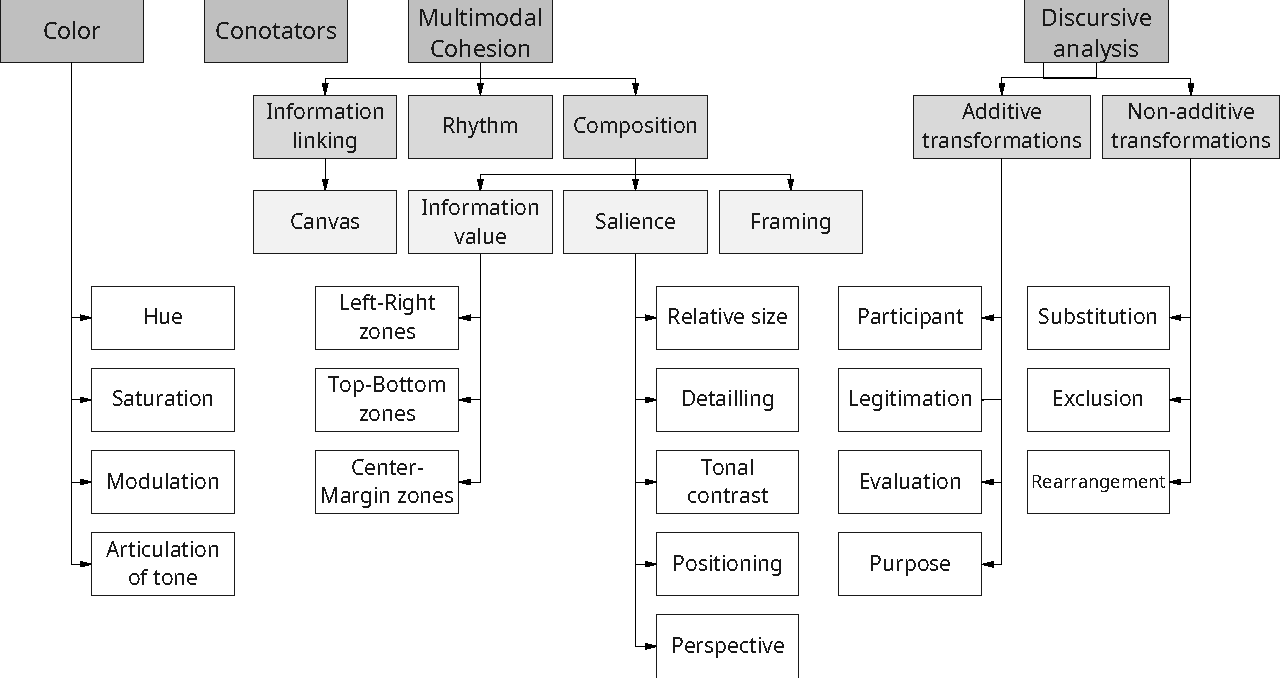
\includegraphics[width=\textwidth]{Fig-1.pdf}
 \caption{Structure of the paper.}
 \label{fig01}
 \source{Created by the authors.}
 \end{minipage}
\end{figure}

\subsection{Color}\label{sec-formato}
Color is a semiotic mode that features semiotic resources such as hue, saturation, modulation, and tonal articulation to create meaning \cite[p. 167]{van_leeuwen_introducing_2005}. In \Cref{chart1}, we present descriptions for each of these resources.


\begin{figure}[htbp]
\begin{minipage}[t]{0.47\textwidth}
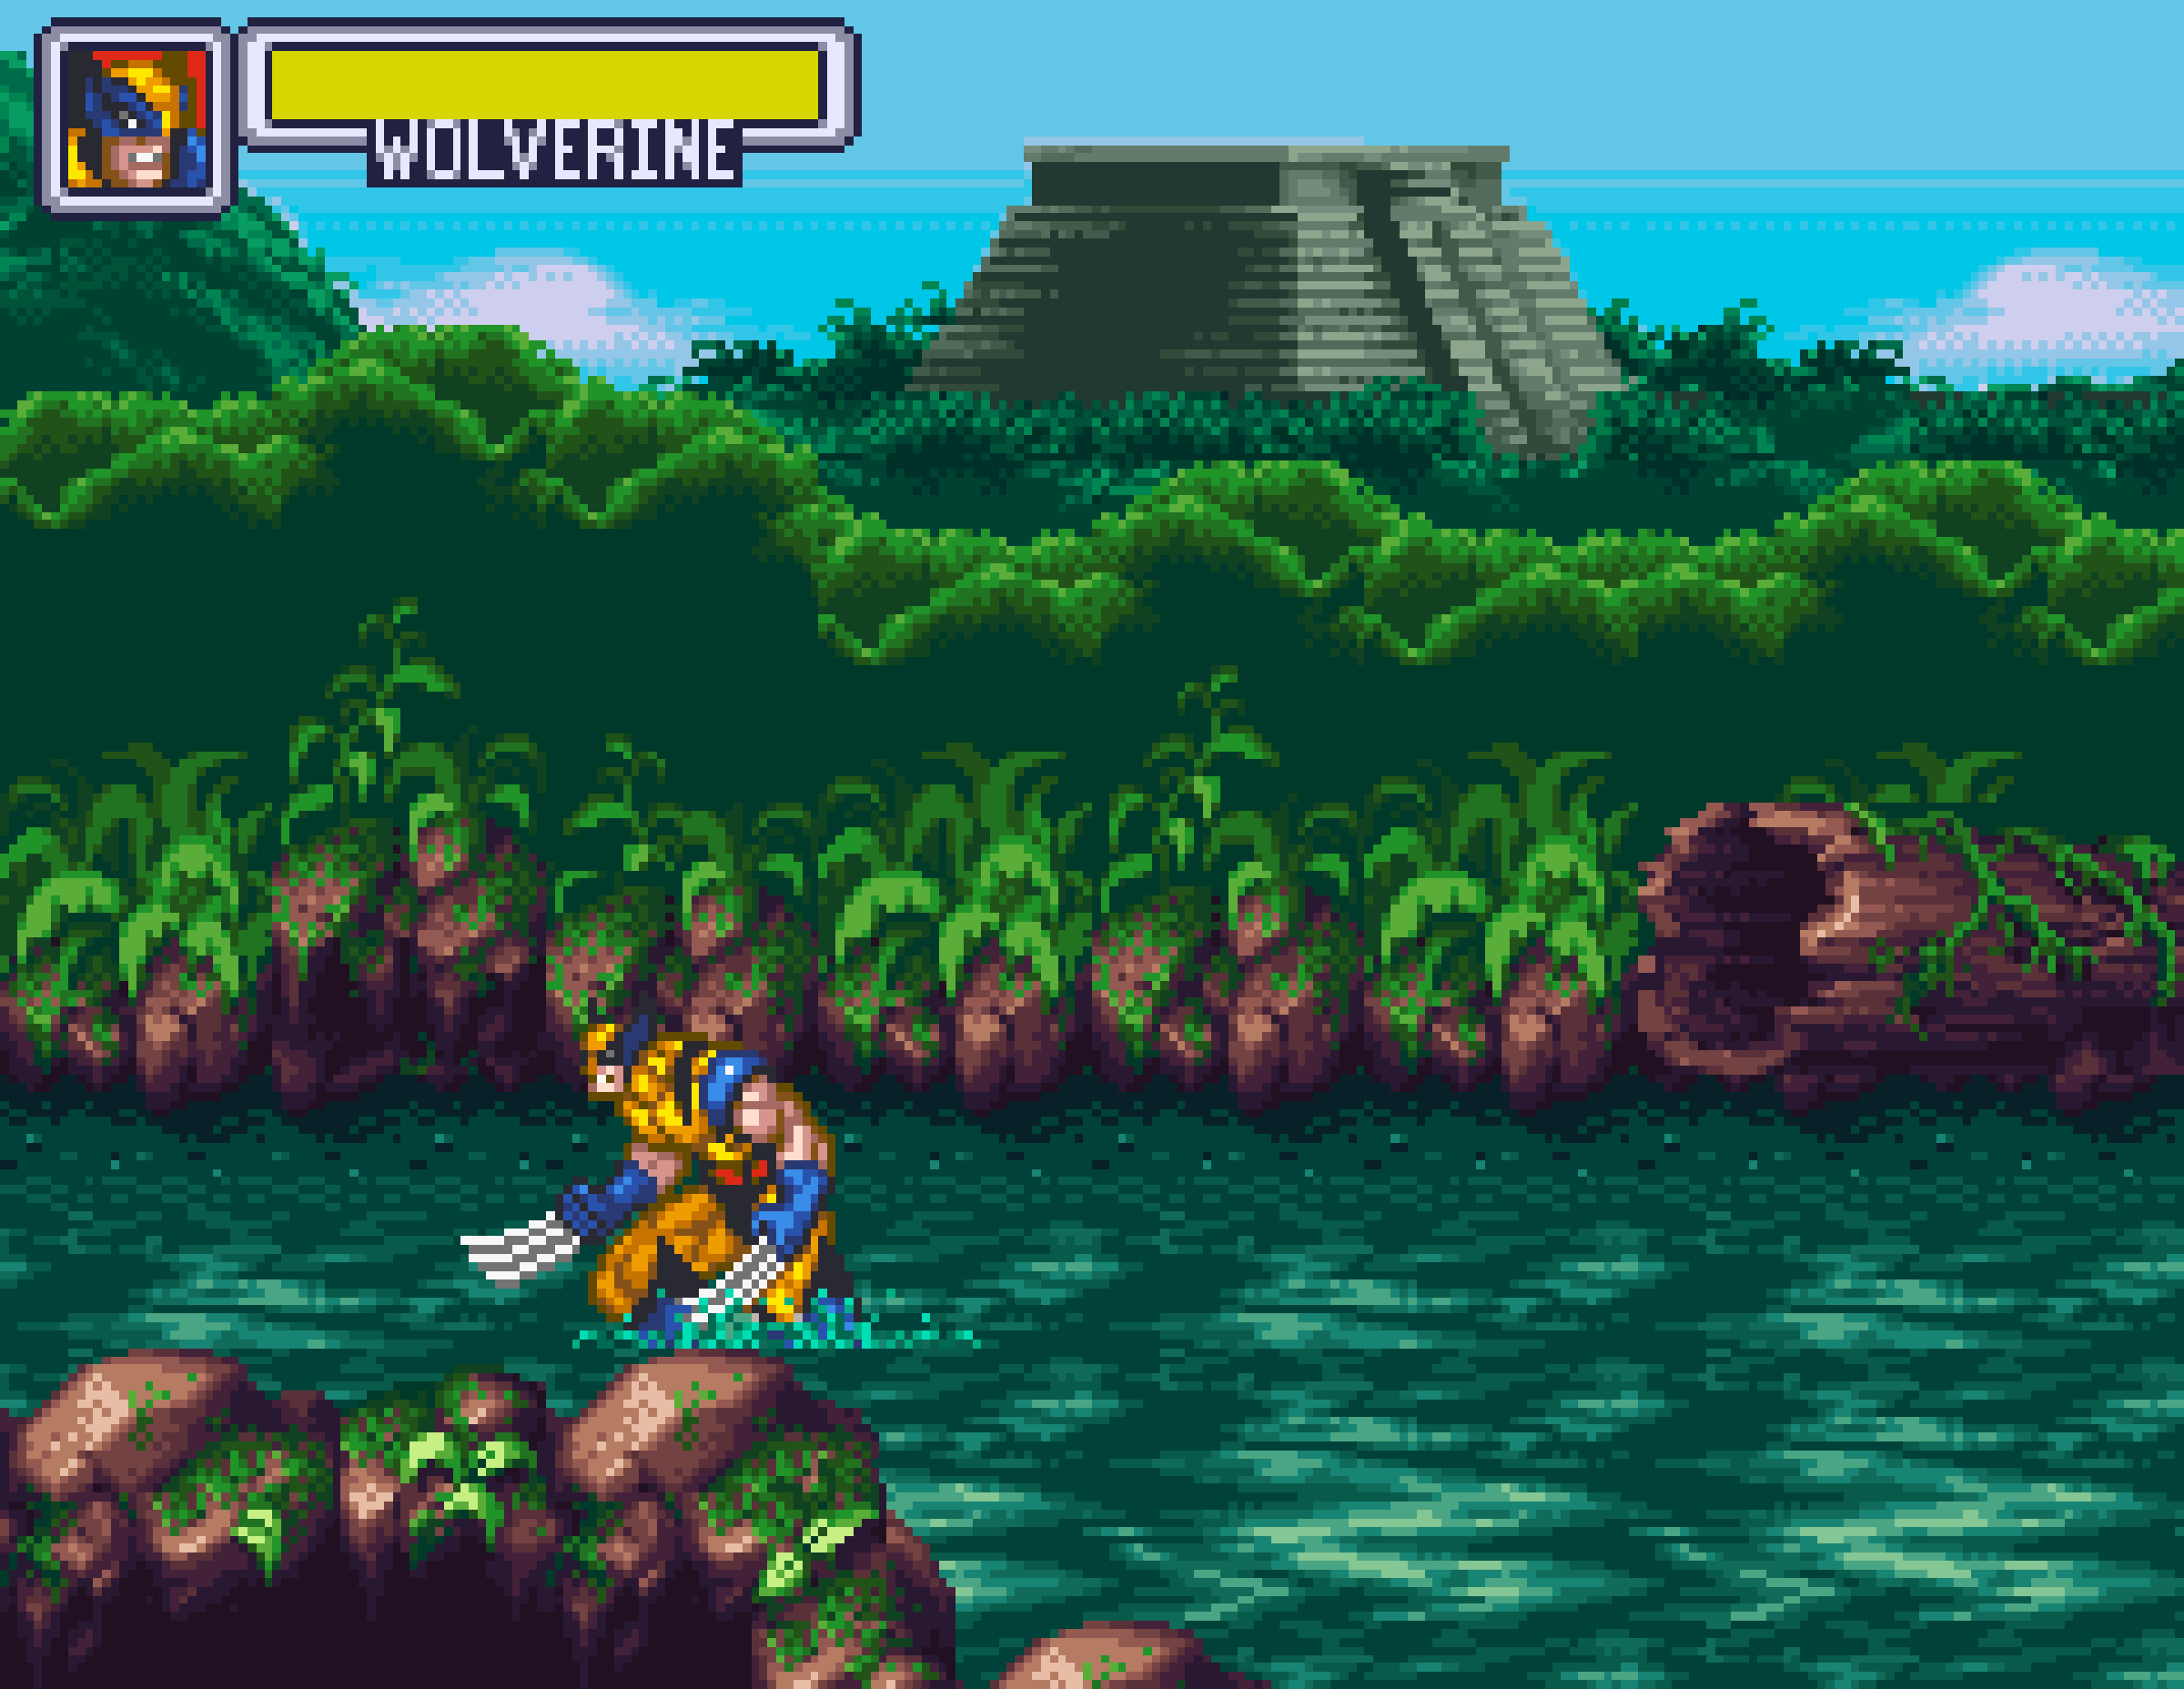
\includegraphics[width=\linewidth]{fig-2a.png}
\subcaption{Wolverine in the Amazonian stage.}
\label{fig2a}
\source{\textcite{capcom_marvel_1996}.}
\end{minipage}
\hfill
\begin{minipage}[t]{0.47\textwidth}
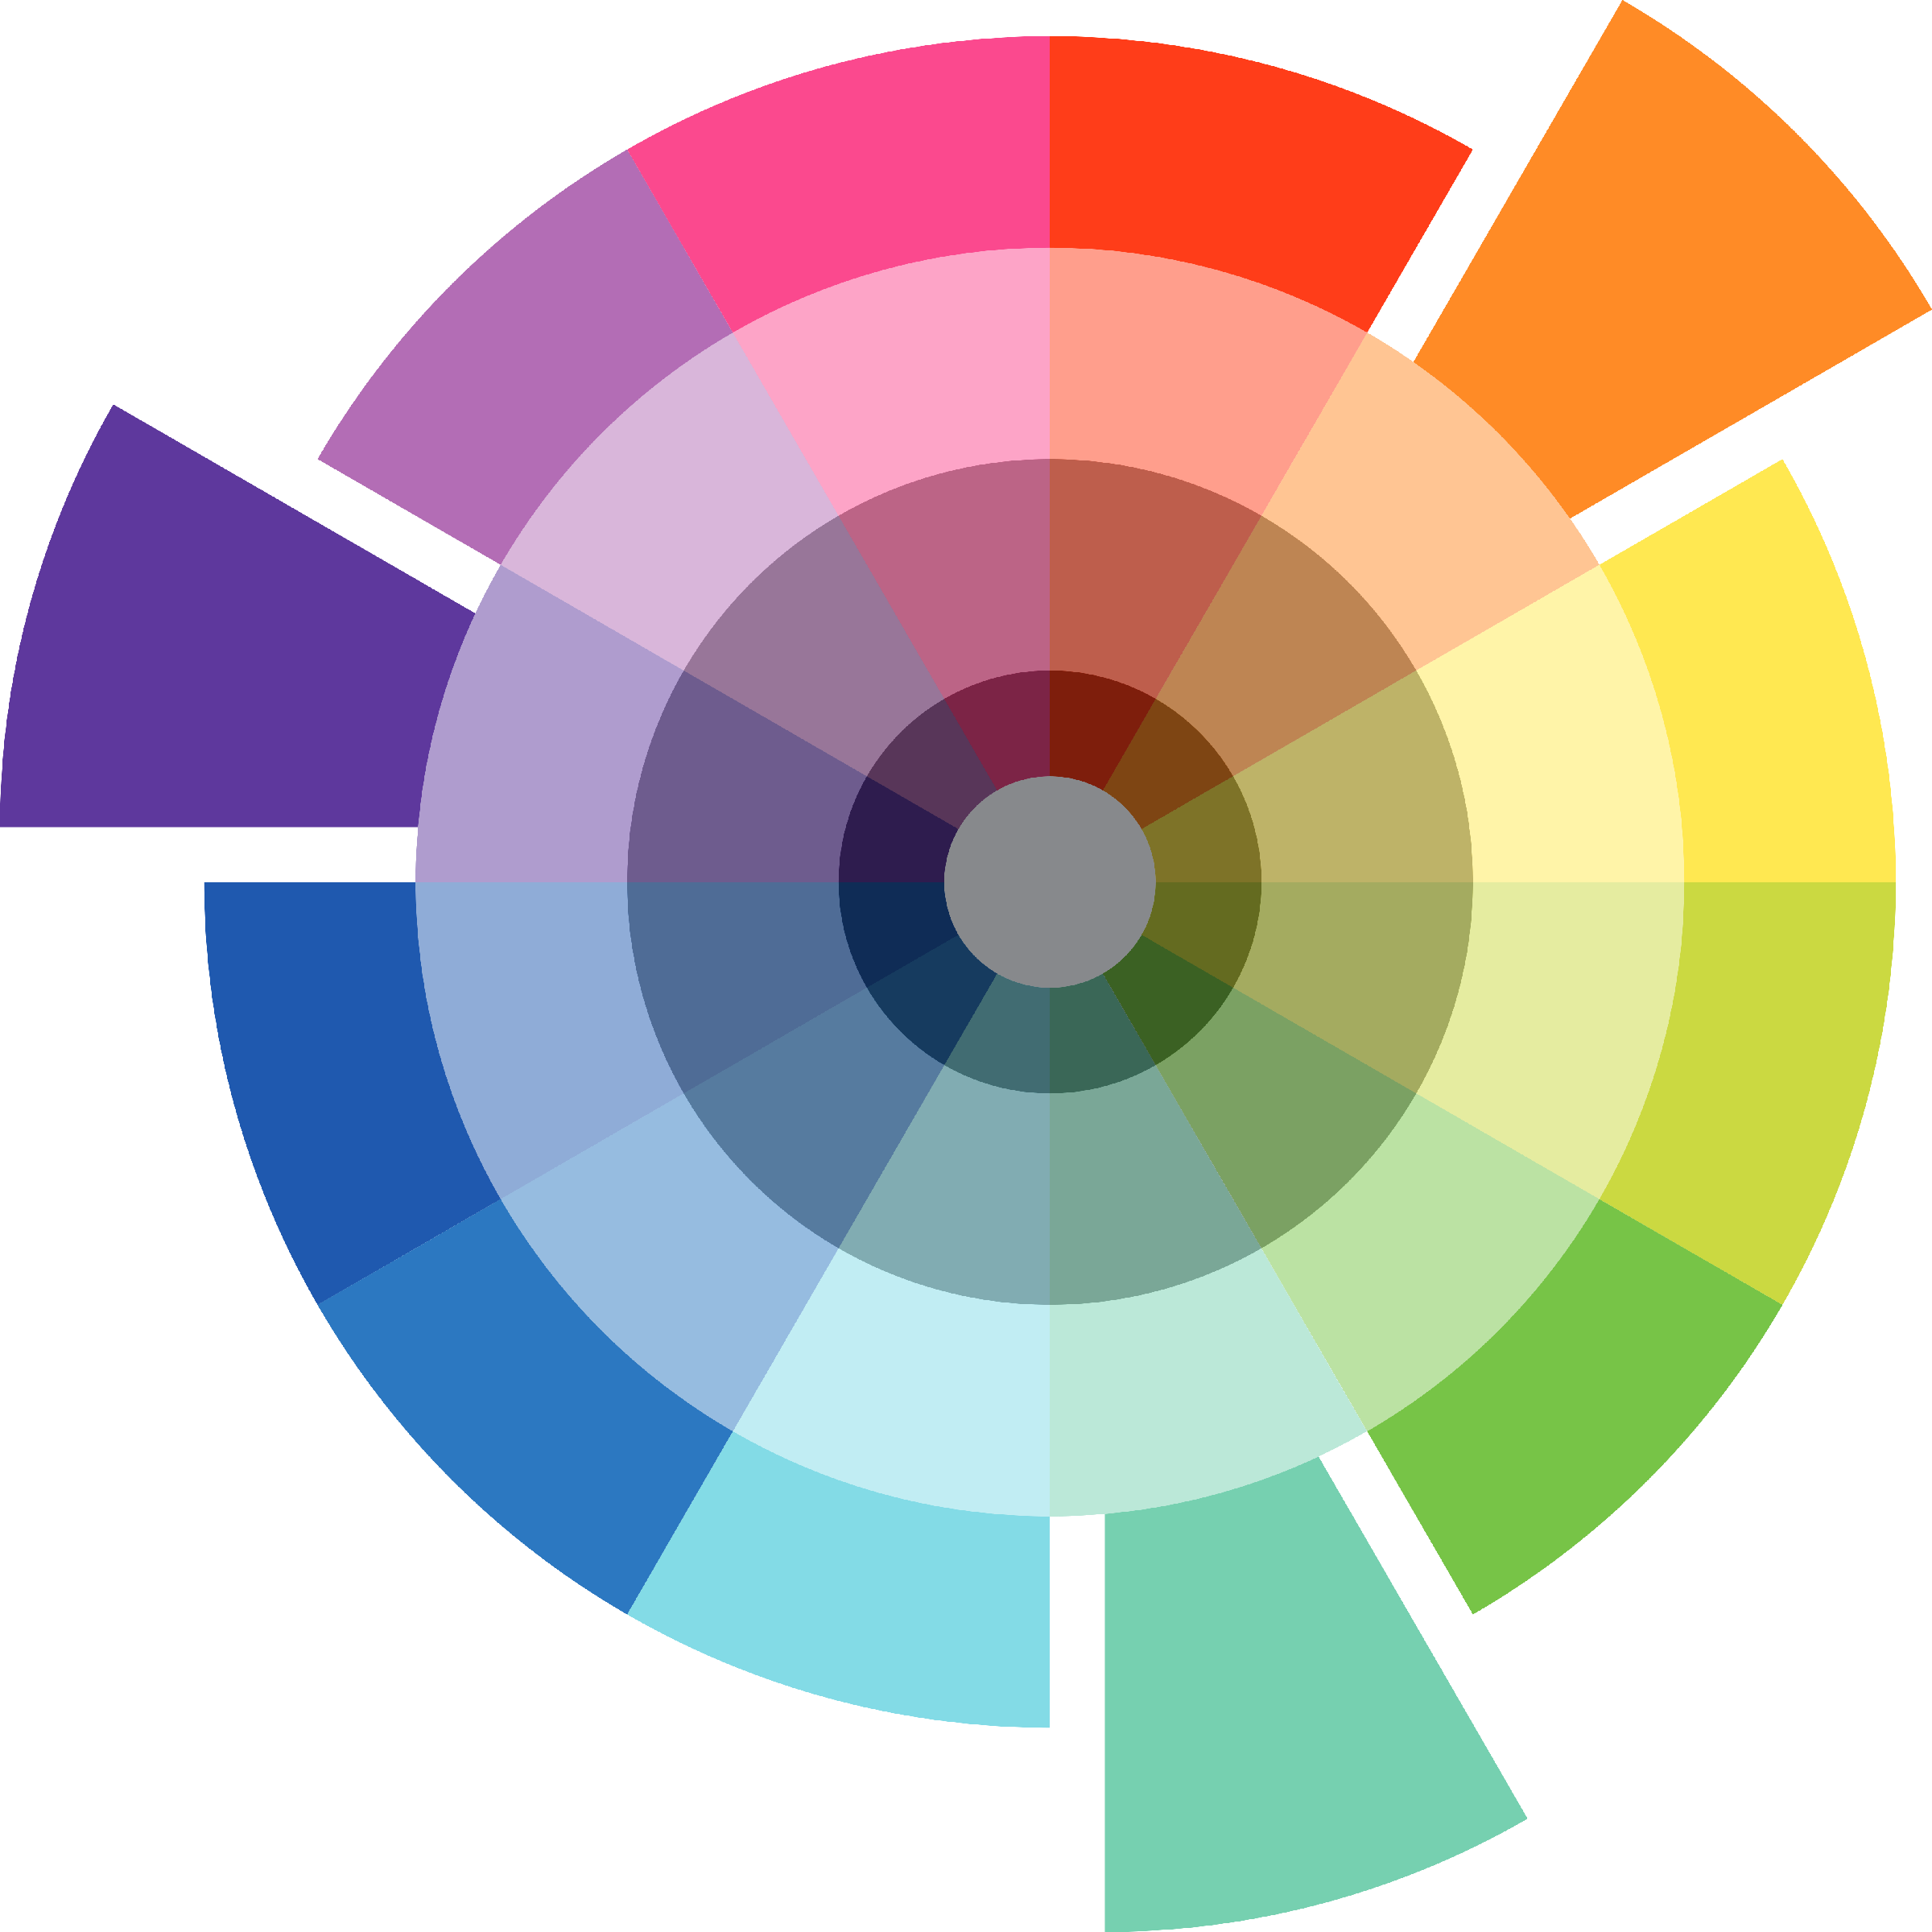
\includegraphics[width=\linewidth]{fig-2b.png}
\subcaption{Color wheel.}
\label{fig2b}
\source{Adapted from \textcite[p. 96]{rhyne_applying_2017}.}
\end{minipage}
\caption{Color’s semiotic resources.}
\label{chart1}
\begin{minipage}[t]{\textwidth}
\small
\vspace{2ex}
\begin{description}
    \item[Hue]: hue is often considered a synonym for color. In colorimetry, however, hue refers to a distinctive feature of color that varies in the RGB (Red, Blue, and Green) scale. Thus, it is possible to describe most colors by their proportions of Red, Green, and Blue. Beyond the individual hues, we can also analyze how they relate to each other by their harmonies\footnote{\textcite[p. 86-97]{rhyne_applying_2017} presents a comprehensive discussion of the possible harmony types and their appliances in digital media.}.
    
    For example, the stage relies on green and brown hues. If we consider brown as the 'key' color — the main color — \cite[p.~86]{rhyne_applying_2017}, 
    it can establish a triadic color scheme with green, as seen on the color wheel on the right (adapted from \textcite[p.~96]{rhyne_applying_2017}).
    A triadic harmony consists of three equidistant colors, one of which is the key color (brown).

    \item[Saturation]:  refers to the range between the lack of colors — black and white — to the maximum saturation of a given color, that is, its purest value \cites[p.~167]{van_leeuwen_introducing_2005}[p.~61–2]{rhyne_applying_2017}.
    We place the purest colors on the outer ring of the color wheel, while the colors inside are mixed with different amounts of gray \cite[p. 61]{rhyne_applying_2017}. In games, it is common to use vibrant colors to make a given participant stand out, be it the player character, a pickup item, or a path to progression.
    
    Another frequent semiotic potential of saturation relates to a metaphor \cite[p. 30]{van_leeuwen_introducing_2005} between saturation and mood: desaturated colors tend to be perceived as sorrowful or downbeat, while vibrant colors tend to be interpreted as happy and upbeat.

    \item[Modulation]: refers to the range between flat colors — less modulated — to the full range of colors within the same hue — more modulated \cite[p. 167]{van_leeuwen_introducing_2005}. In \textit{Marvel Super Heroes}, the forest has only a couple of green hues, enough to differentiate parts of the vegetation but lacking in detail. Conversely, the yellow hues in Wolverine’s clothes create outlines, shadows, and light reflection, which makes the character more detailed compared to the background.

    \item[Articulation of tone]: also called \textit{Brightness}, refers to the range between monotone colors to brighter or darker tonalities within the same hue \cites[p. 167]{van_leeuwen_introducing_2005}. The color of the river conveys movement and reflection through the use of darker shades of green-blue against the lighter highlights within the same green-blue hue.
\end{description}
\end{minipage}
\source{Left image created by \textcite{capcom_marvel_1996}; color wheel adapted from \textcite[p. 61]{rhyne_applying_2017}; chart created by the authors.}
\end{figure}

\subsection{Connotators}\label{sec-modelo}
The categories in this section relate to denotative and connotative meanings. The denotative component of an image refers to what is effectively depicted \cite[p. 23]{ledin_introduction_2007}. Although we usually assume that it is synonymous with ‘reality,’ we emphasize that the choices made by the sign maker can limit or enhance the potential meanings conveyed by an image \textcite[p. 23]{ledin_introduction_2007}. The connotative component, on the other hand, refers to the associations that any given participant may evoke \cite[p. 219]{machin_how_2012}. Let us take Mario from the Super Mario series as an example: Mario is an Italian plumber with a big nose, a mustache, a red cap, a red shirt and blue dungarees. To convey (connote) his profession, the creators used the dungarees, which can be associated with physical labor, while his Italian origin is based on the association between Mario's physical features and a stereotypical representation of an Italian chef.

Based on this example, we can draw three conclusions. The first is that every visual participant has connotative meaning potential. We are not lost in a sea of endless possibilities, however: usually, the creator leaves ‘clues’ that lead us to the intended meaning. This does not mean that we always interpret an image as the creator intended, but rather that some meanings are eliminated during the image making process. Second, connotative meanings are socially constructed; they depend on the context in which they are inserted \cite[p. 219]{machin_how_2012}. Mario's creators thus rely on an image that they consider among the players as a signifier of the 'Italian worker.' The third and final conclusion is that we can signify ideas and values associated with the original context of the image by importing signs from that context. This is called Provenance \cite[p. 10]{kress_multimodal_2001}.

Connotators, then, are predetermined carriers of connotations that are assumed to be capable of conveying certain meaning(s) \cite[p. 51]{machin_how_2012}. Flags, for example, are connotators: when we see the U.S. flag, it is denotatively a rectangular shape with white stars, a blue square in the upper left corner, and red-white stripes that cover almost the whole rectangular shape. Connotatively, depending on the context, numerous associations with the U.S. flag can arise: hoisted on the outside of a house, it can symbolize the patriotism of the owner; at the Olympics, it represents the U.S. athletes who then represent their country.

To analyze the connotative potential of games, we must consider them as texts embedded in a sociocultural context and in a network of interrelated texts. As an example of this, we can take the pyramid in \textit{Marvel Super Heroes} Amazon stage. The game depicts it as part of Brazil, but it looks exactly like the \textit{El Castillo} or the Temple of Kukulkan in \textit{Chichén Itzá}, Yucatán, Mexico \cite{proskouriakoff_album_2003}.

Before we continue the discussion, it is important to point out that the game does represent Brazil, even if its representation does not perfectly correspond to the country. Each representation is a semiotic ensemble of resources and participants that may or may not correspond to its real counterpart. Thus, we should critically analyze these choices by considering their meaning-making processes within the game and as broader signifiers of the context and ideologies that the game may convey.

That said, we can make a hypothesis about what the connection between Brazil and Mexico is. First, they are both from Latin America; second, they have a common colonial past, even if Brazil was a Portuguese colony, while Mexico was a Spanish colony. However, it seems unlikely that this was the driving force behind the choice, as there is no colonialist iconography or mention in the game. Thus, we propose a more subjective association: in media, from cinema to video games, it is common to portray other cultures as the 'other.' This 'other' can have positive or negative connotations, often by ‘vesting’ them of ideas that are foreign to them but seen as fitting to them by the creators. This leads to stereotyping, i.e., simplifying the 'other' to a few easily readable characteristics \cite[p. 257]{hall_spectacle_1997}.

In \textit{Marvel Super Heroes}, the game conflates the image of the Amazon Forest with the 'ancient' Peoples of Mesoamerica, which include the Mayans. Just as Mexico and Brazil can be lumped together under one heading, the Amazon and its People are lumped together with many other parts of the Americas. As mentioned earlier, stereotypes simplify cultures. Therefore, they are 'essentialized' as identical; their spaces iconography become interchangeable.

To conclude this section, we propose to extend the visual analysis of video games by considering the connotative meanings and connotators that these artifacts carry. This allows the analyst to examine the intertextuality between different games, rather than viewing the visual choices as a singular thing. For example, Mesoamerican Pyramids are also present in Mega Man X6 \cite{capcom_mega_2001} in Commander Yammark's stage, the Amazon Area, while in games such as Real Bout Fatal Fury Special \cite{snk_real_1997} and Street Fighter III: new generation \cite{capcom_street_1997} Atlantean Figures, statues built by the Toltecs, another Mesoamerican People \cite[p. 17, 202]{aguilar-moreno_handbook_2006}; \cite[p. 42, 400]{evans_ancient_2013} are represented as part of Brazilian iconography. Thus, there is a tradition of Mesoamerican iconography to signify the Amazon Forest (and Brazil in general) that can only be traced through intertextual analysis.

\subsection{Multimodal cohesion}\label{sec-organizacao}
Multimodal cohesion refers to the way semiotic resources and modes are integrated to form multimodal texts \cite[p. 179]{van_leeuwen_introducing_2005}. Here, we will focus on the relationship between the visual mode and the other modes used in the game.

\subsubsection{Information linking}\label{sec-organizacao-latex}
Information linking refers to how semiotic items "can be and are meaningfully linked to other items of information" \cite[p.~219]{van_leeuwen_introducing_2005}. There are many ways to link modes, such as chronologically or logically. \textcite[p.~219-47]{van_leeuwen_introducing_2005} proposes a scheme for linking analysis in which the relevant semiotic modes are arranged in parallel to determine intersections and connection points between bits of information.

\begin{figure}[htbp]
 \centering
 \begin{minipage}{.95\textwidth}
 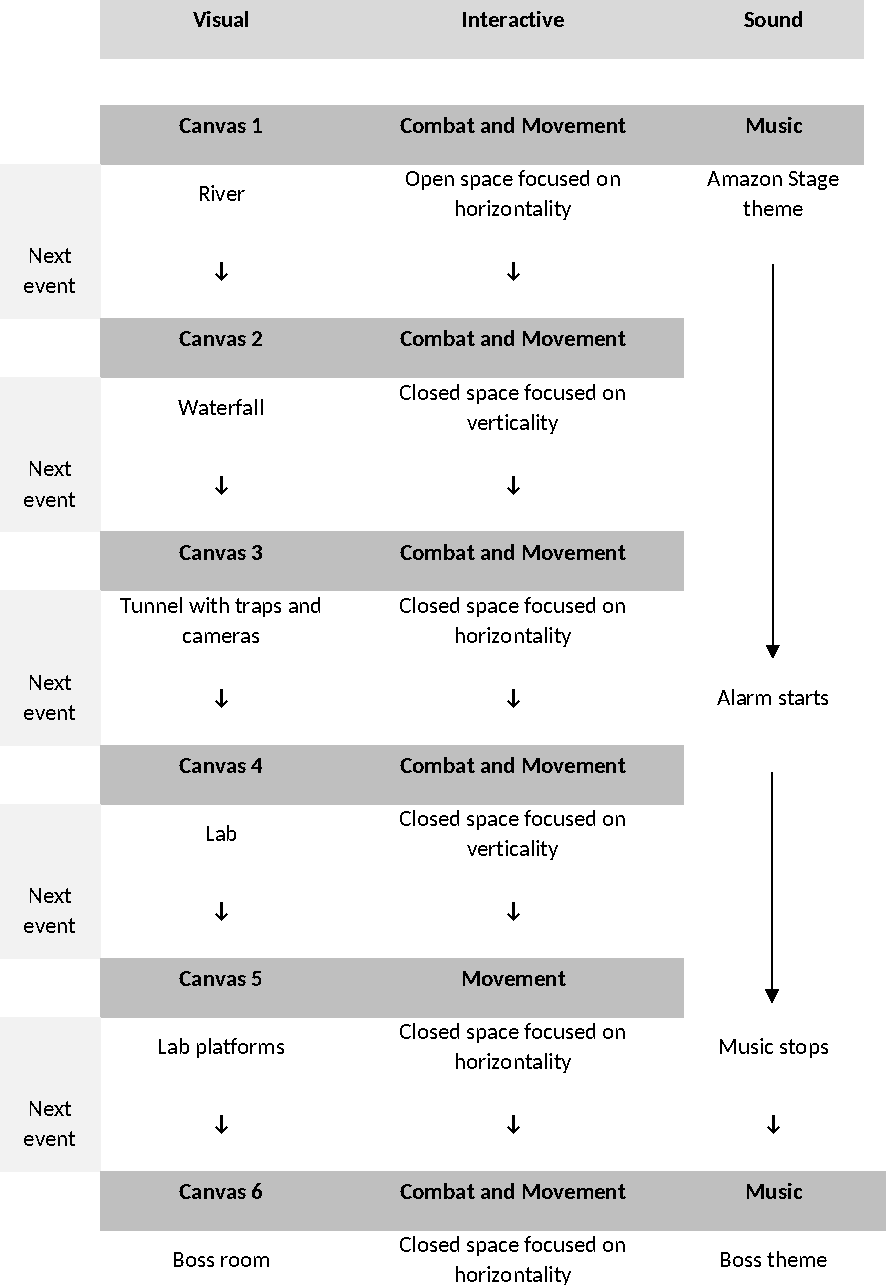
\includegraphics[width=\textwidth]{fig-3.pdf}
 \caption{Information linking in \textit{Marvel Super Heroes in War of the Gems}.}
 \label{fig03}
 \source{Created by the authors.}
 \end{minipage}
\end{figure}

In \Cref{fig03}, we compared image, sound, and interaction. For games like \textit{Marvel Super Heroes}, this linear representation is appropriate because players have little freedom to explore the stage, even though the way they traverse this space may vary. For games with more variables, we can rely on the interactive linking framework proposed by \textcite[p. 237]{van_leeuwen_introducing_2005} for websites and other link-based texts.

Based on the scheme, we can extrapolate how the player's choice overlaps with semiosis. To better organize this type of analysis, we resort to the concept of 'Canvas.' \textcite[p. 101]{bateman_multimodality:_2017} define it as the "locus of semiotic activity," "the interface that a medium provides for the interpreters of the 'messages' that the medium carries." Canvas can be simple or complex in structure. In complex structures, a Canvas is "articulated in subcanvases of various kinds." Thus, the individual screens of the game — to which the player currently has access — are subcanvases of the visually-themed Canvases\footnote{The authors utilize the concept of Canvas multimodally, while we will restrict it only to the visual mode.} we proposed in \Cref{fig2a}.

In Canvas 1, for example, enemy forces repeatedly stop the player from progressing. These ‘mini-events,’ or subcanvases, are essentially the same thing, and as such we consider them parts of a larger event, or Canvas.

The tag 'next event' indicates a temporal sequence; each 'event' follows the next chronologically \cite[p. 225]{van_leeuwen_introducing_2005}. It is worth noting that there is also a spatial connection between scenes as the player moves between them. However, since there are no cuts between scenes, we chose to examine gameplay as a temporal event.

Next, for the interactive dimension, we proposed a system with three variables: (i) combat-movement; (ii) open-closed spaces, and (iii) verticality-horizontality. For the combat-movement system, we focus on the main task the player has to fulfill. This means that although combat and movement often occur together, we emphasize the action most important to progress. Open and closed spaces refer to how space constrains or enables the player's actions. It is worth noting that the openness of the space does not refer so much to how the stage is presented, but rather to how the player can interact with the environment. In this sense, a stage can be represented as an open environment, but the player has very little room to move and interact. Conversely, a space that is represented as closed can allow the player free movement and interaction. Put simply, we can refer to the representational side as \textit{semiosis} and the interactive side as \textit{ludosis} \cite[p. 19]{mayra_introduction_2008}. Finally, verticality and horizontality emphasize the relationship between action and space: we analyze the orientation of the screen and how the player must overcome obstacles. Thus, a horizontal orientation can evoke actions such as running or walking, while a vertical orientation can evoke actions such as jumping or climbing.

Finally, the sound mode consists of music and sound effects, such as punch sounds. Additionally, in Canvas 3, an alarm intersperses the Amazon Forest music, while in the last part of the stage (Canvas 6), the Boss theme is played. Unlike the musical theme of the stage, all the bosses have the same music.

\Cref{fig-4,fig-5ae5b,fig-6ae6b,fig-7,fig-8,fig-9}
highlights these moments and underscores the multimodal ensemble that the game employs at the Amazon Forest stage.

\begin{figure}[htbp]
\begin{minipage}[t]{.47\textwidth}
\vspace{0pt}
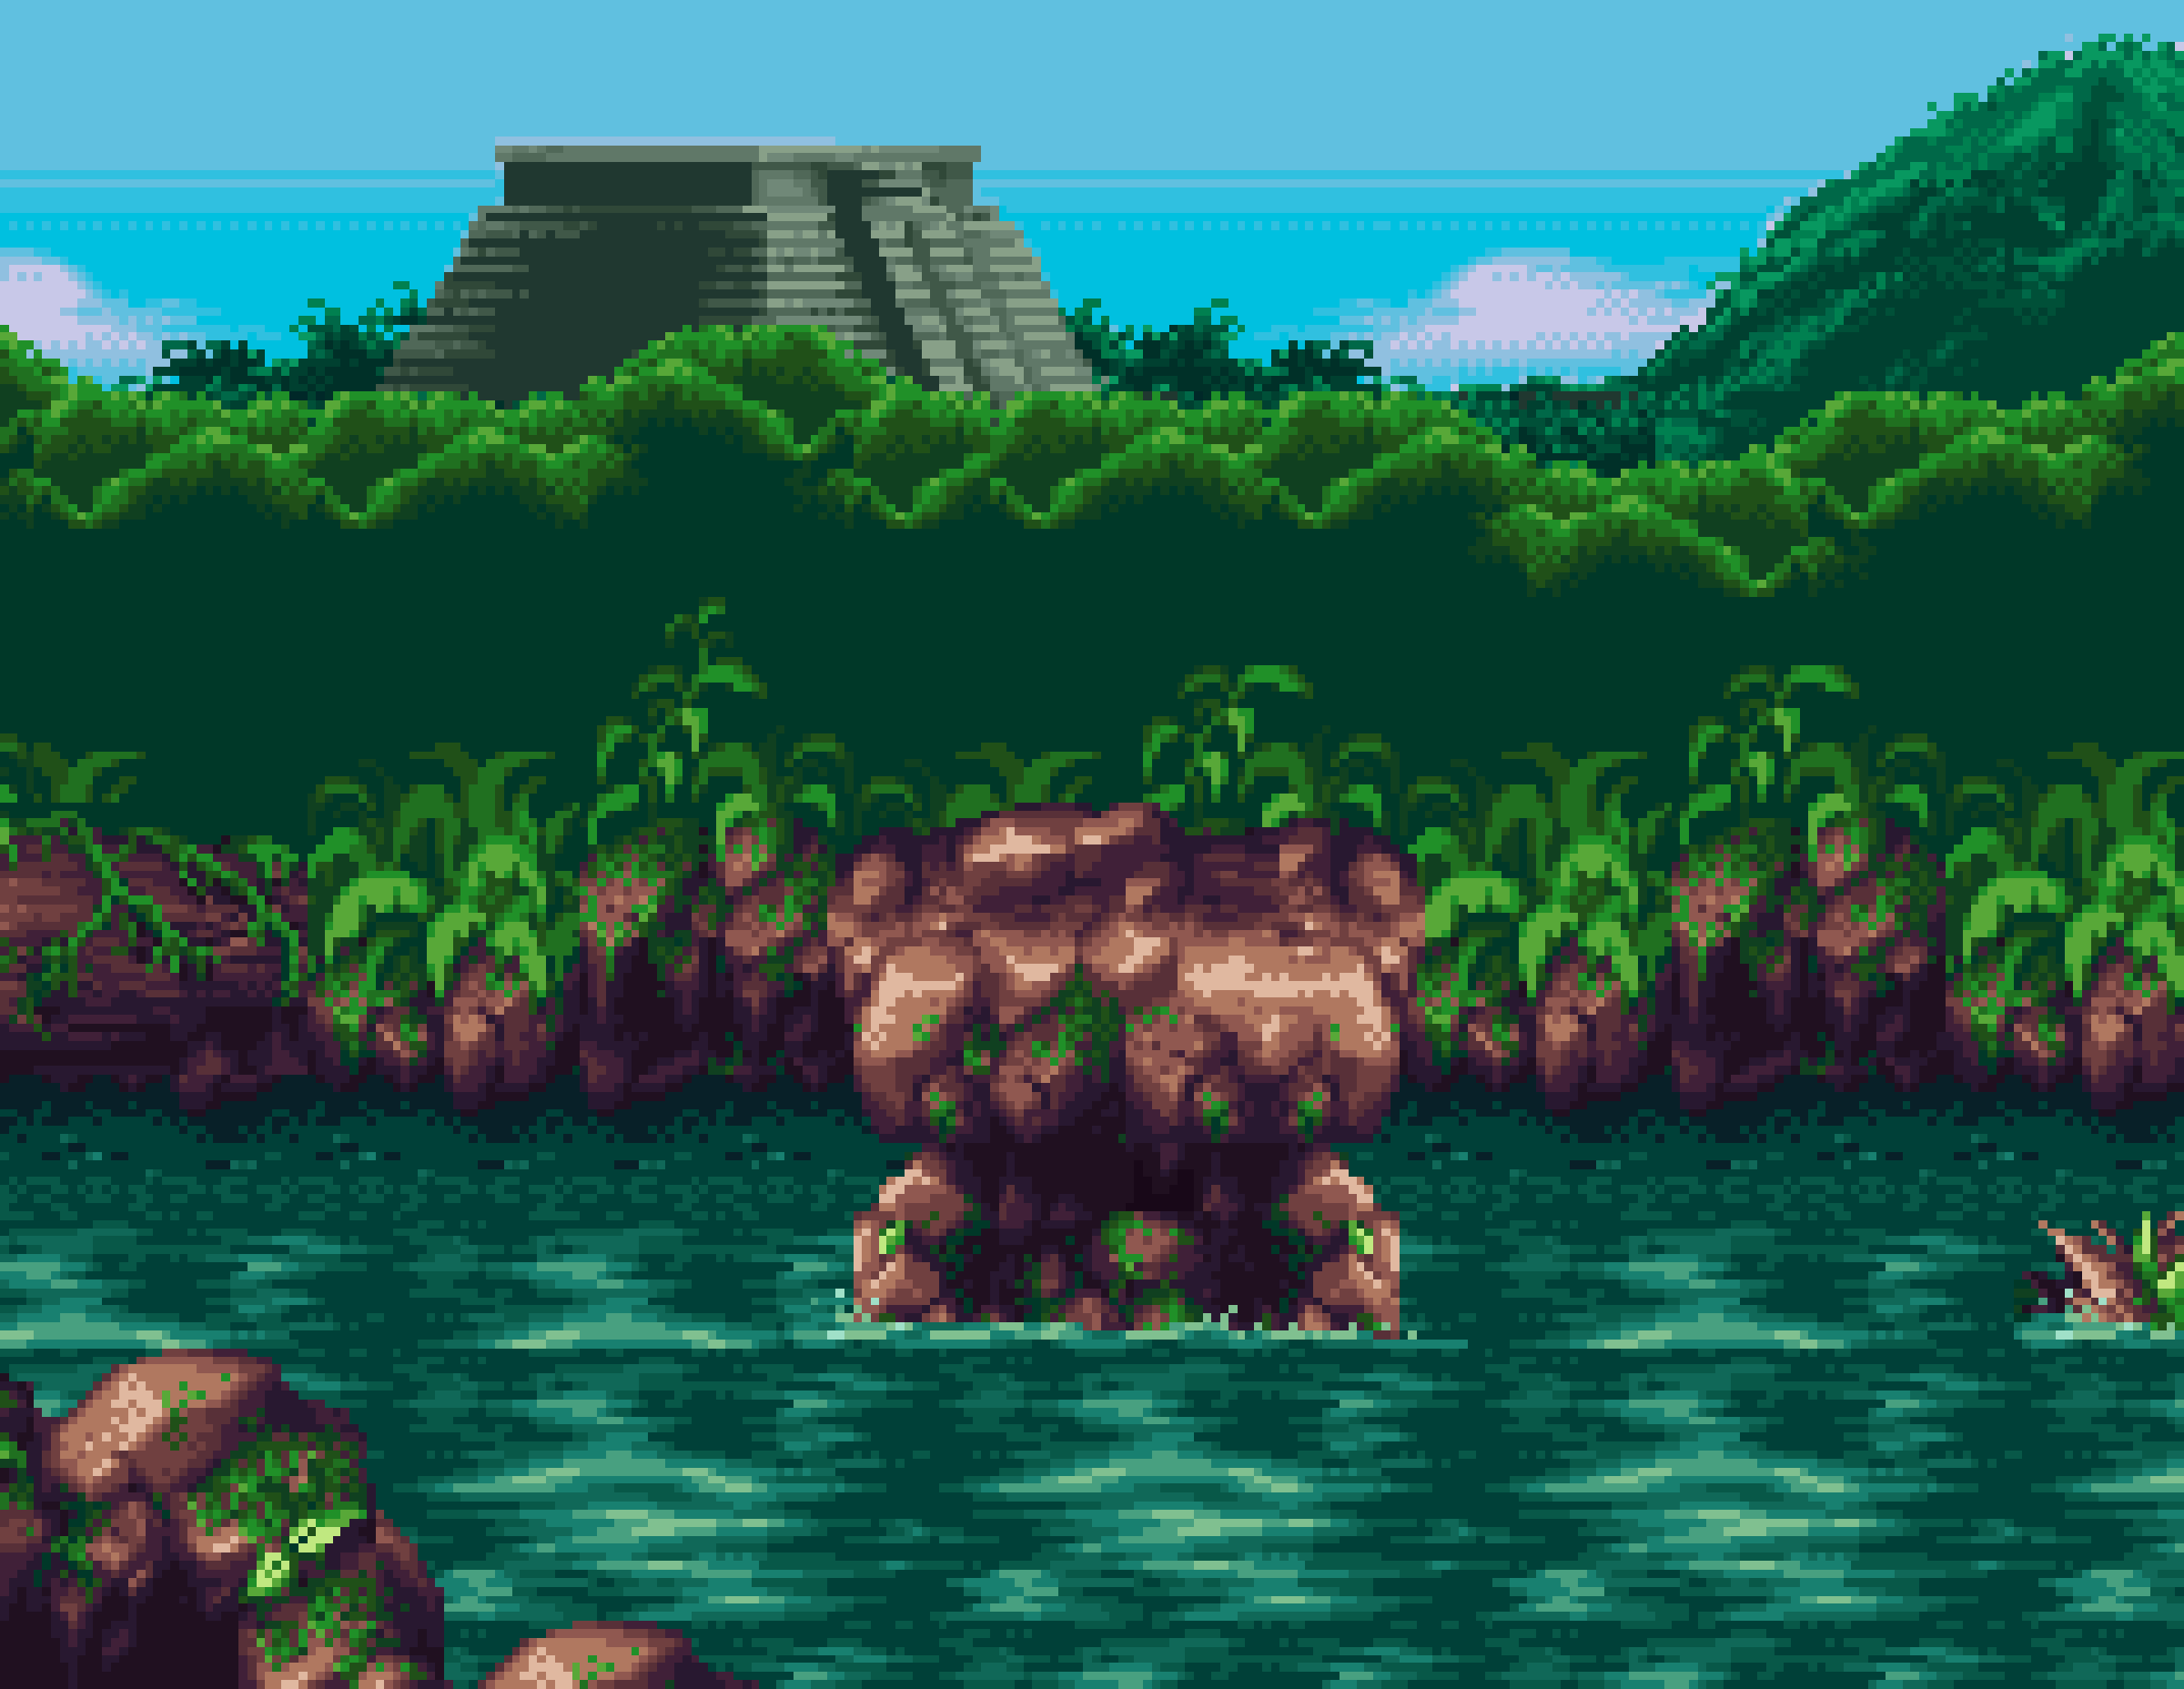
\includegraphics[width=\textwidth]{fig-4.png}
\caption{Forest.}
\label{fig-4}
\source{\textcite{capcom_marvel_1996}.}
\end{minipage}
\hfill
\begin{minipage}[t]{.47\textwidth}
\vspace{2pt}
\textbf{Canvas 1}, 'Forest': the player starts the stage at the Amazon River. The player moves to the right, in the same direction that the river flows. In this Canvas, ground and aerial enemies attack them. The player will also find rock platforms (center of the figure) and spiky plants (right edge of the figure). The platforms help fight the enemies from the air, while the spiky plants hurt the player.
\end{minipage}
\end{figure}

\begin{figure}[htbp]
\begin{minipage}[t]{.47\textwidth}
\vspace{0pt}
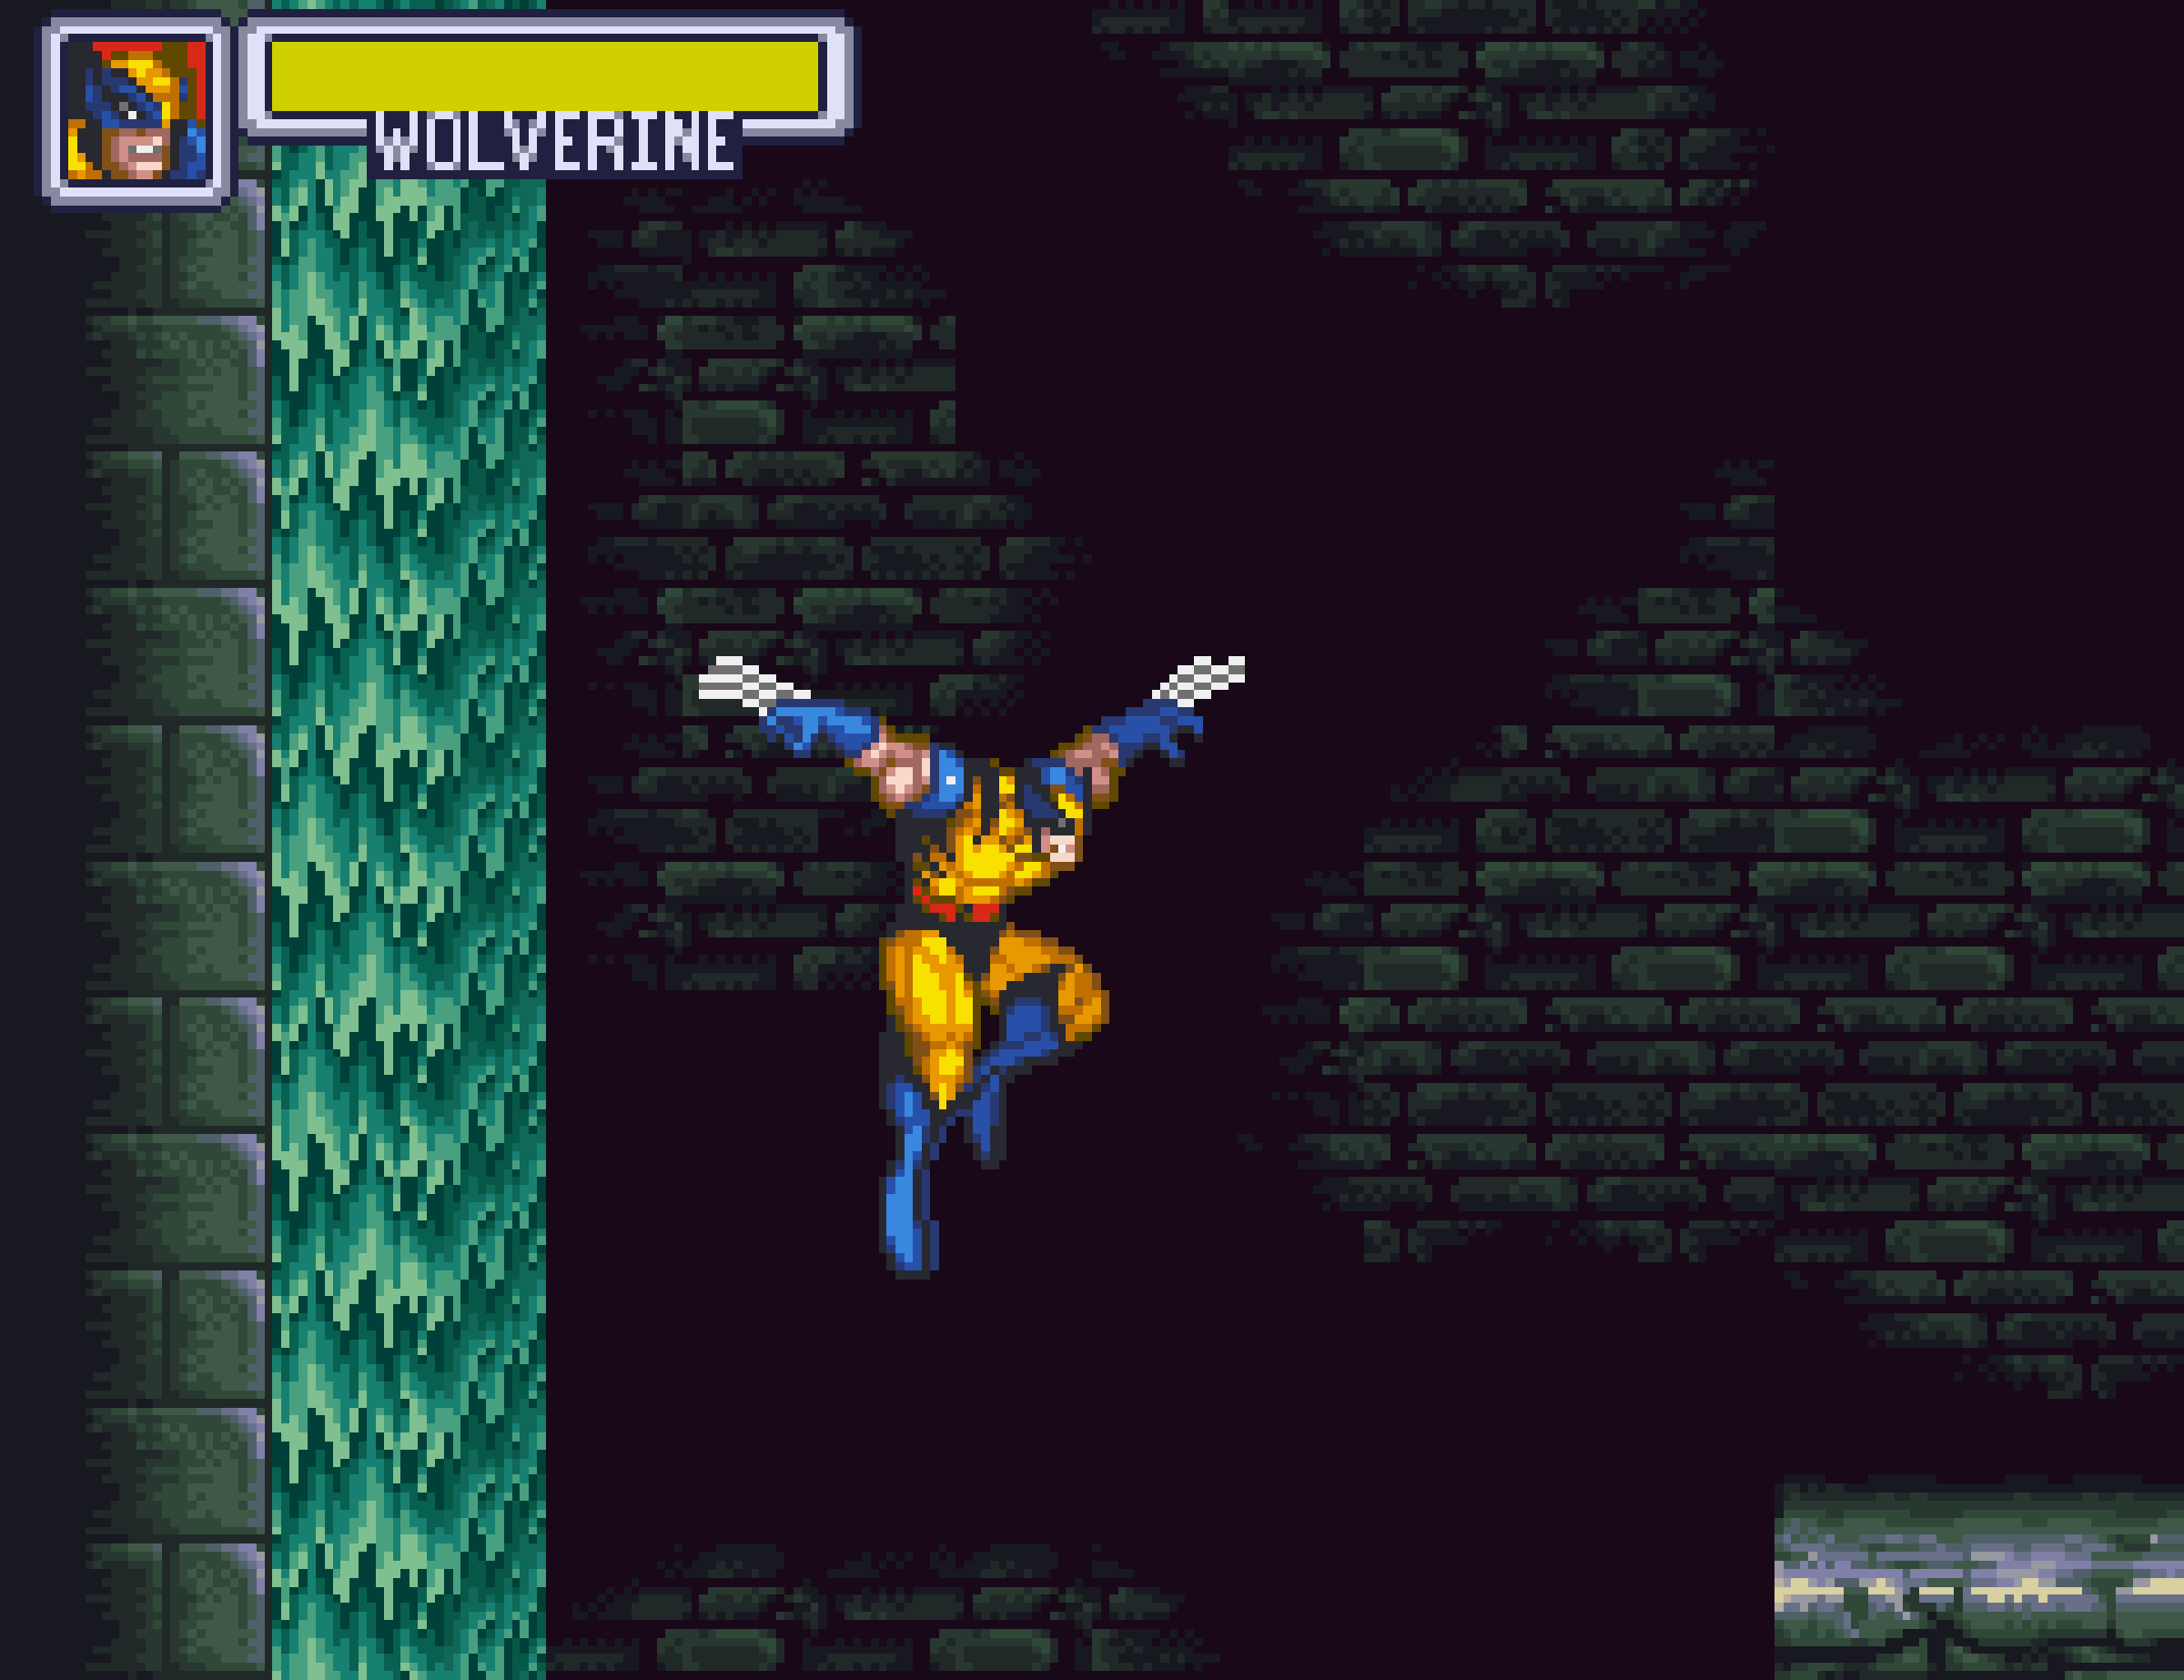
\includegraphics[width=0.49\textwidth]{fig-5a.png}
\hfill
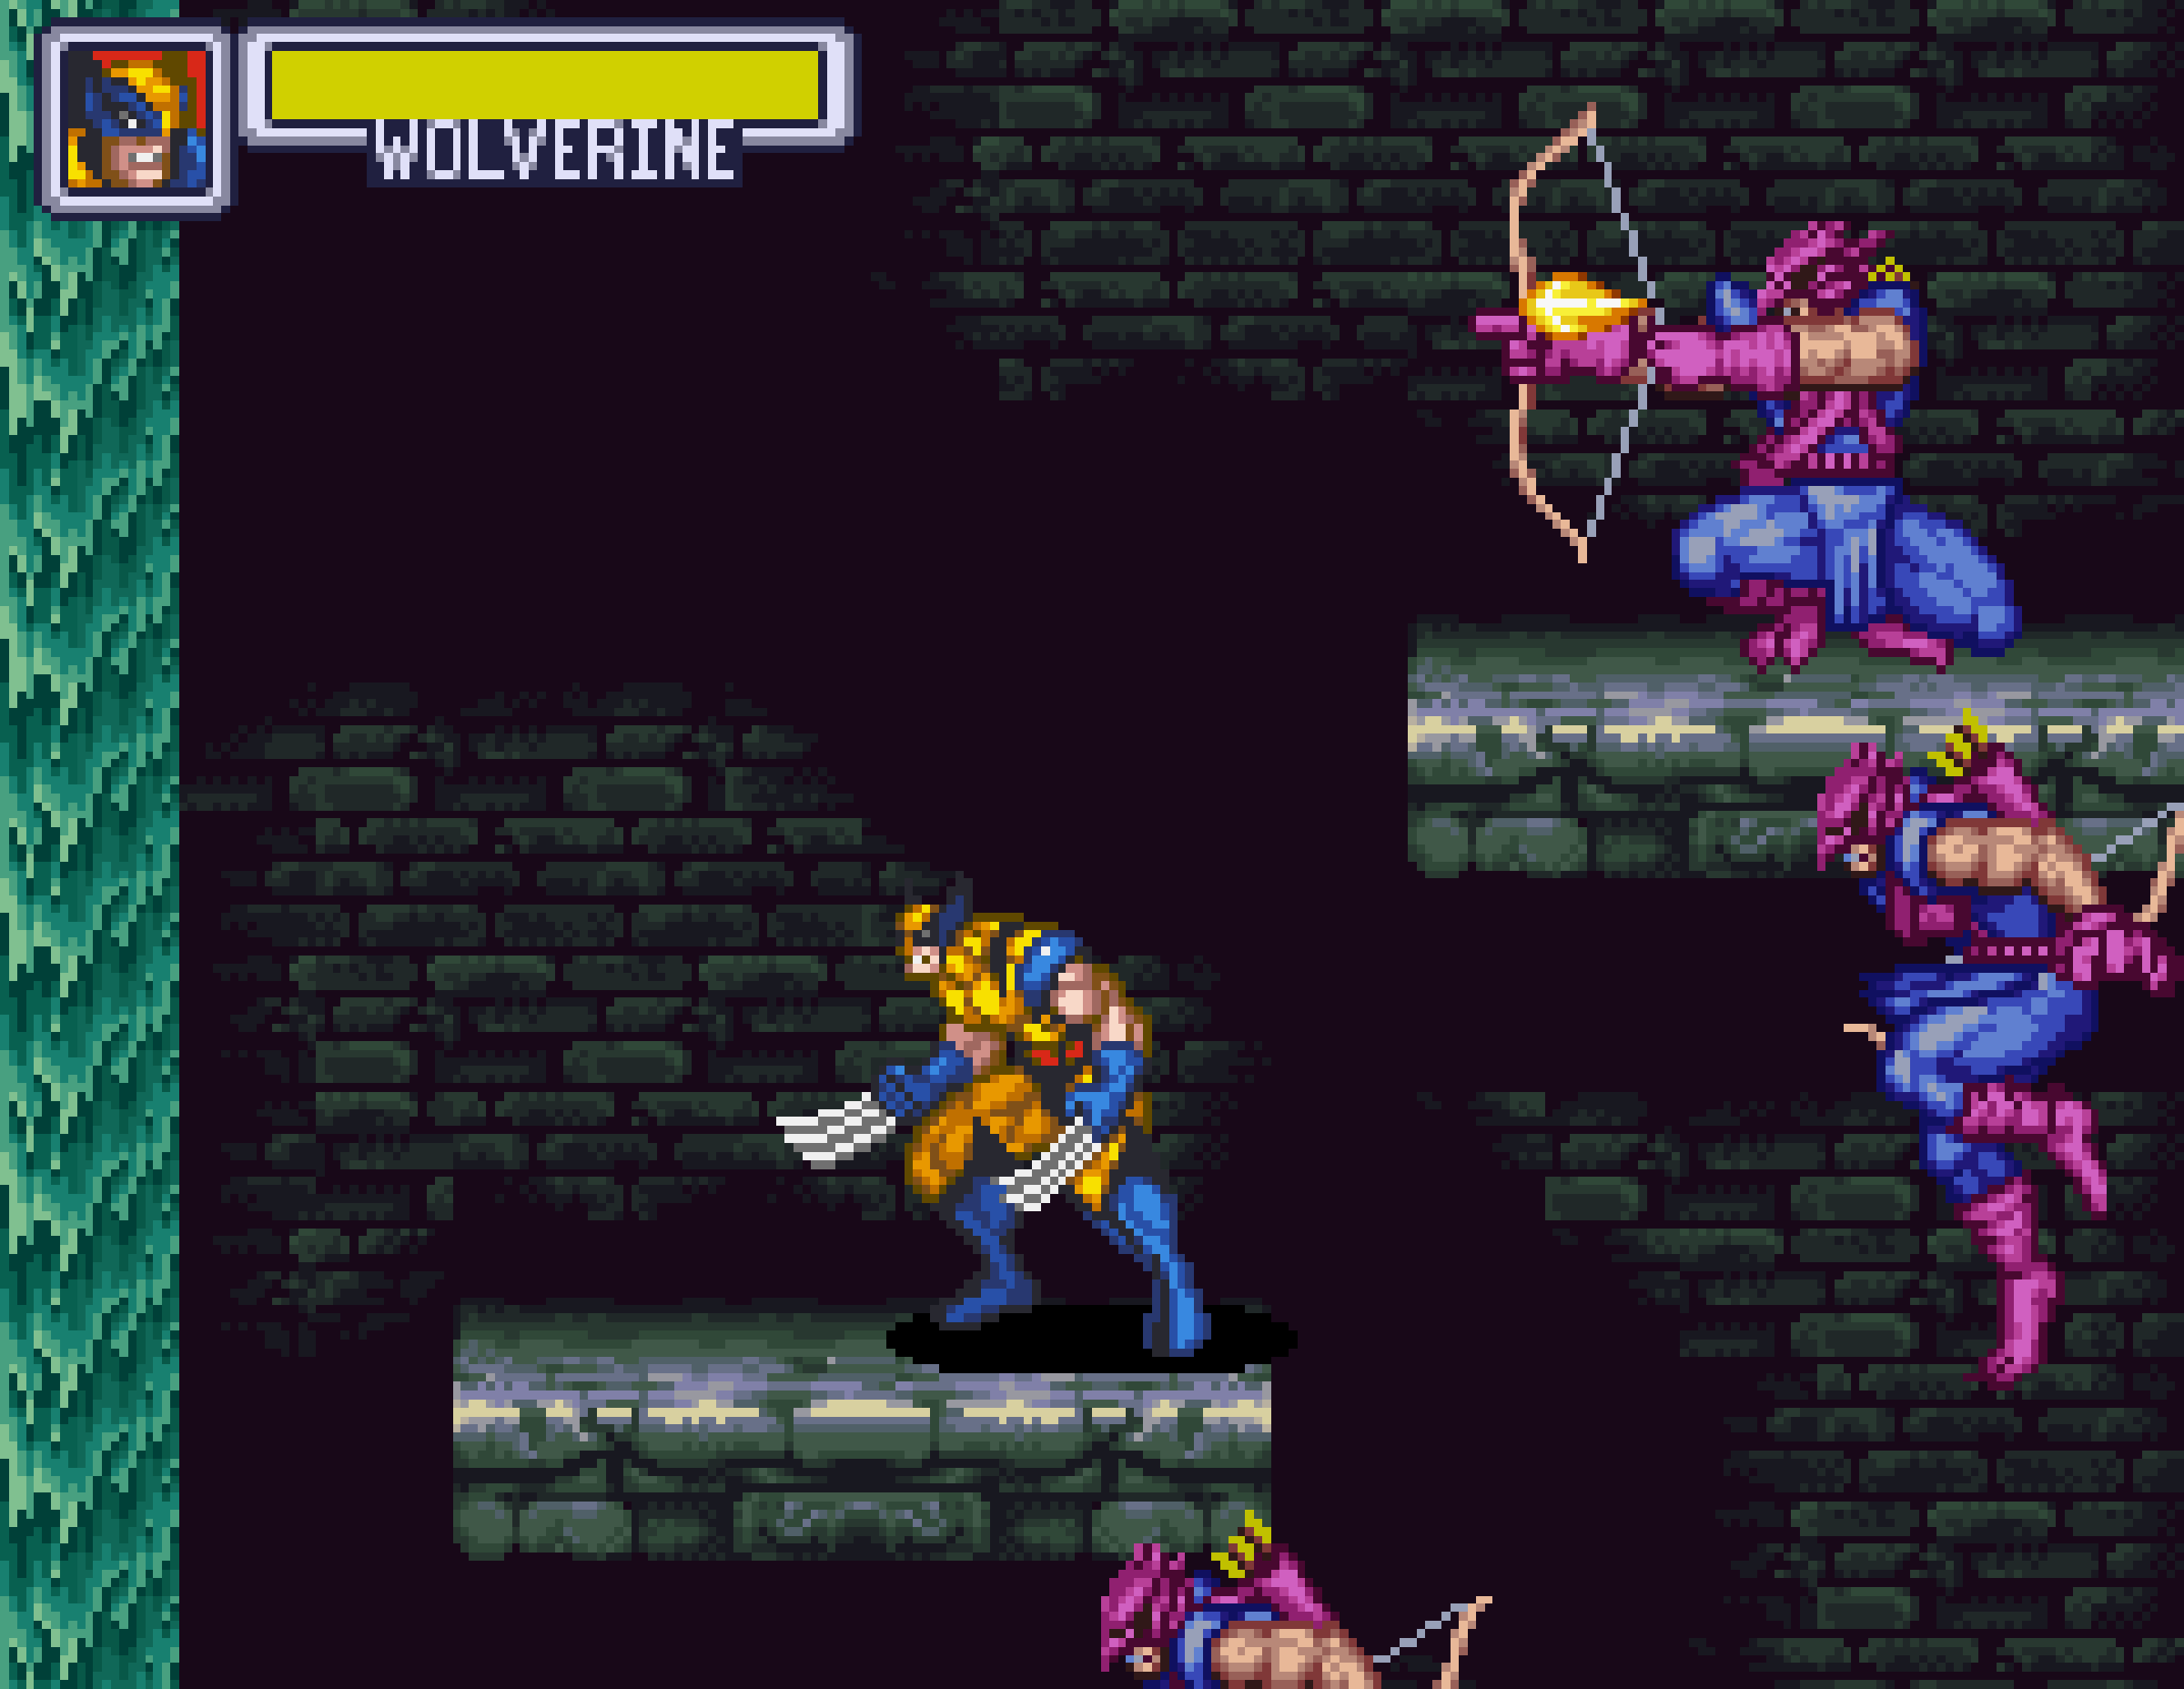
\includegraphics[width=0.49\textwidth]{fig-5b.png}
\caption{Waterfall.}
\label{fig-5ae5b}
\source{\textcite{capcom_marvel_1996}.}
\end{minipage}
\hfill
\begin{minipage}[t]{.47\textwidth}
\vspace{2pt}
\textbf{Canvas 2}, 'Waterfall': a waterfall connects the river to the lower parts of the level — the ruins mentioned in the level description. A group of archer enemies appears and attacks the player from a distance. The player must move across vertical platforms to deal with the threat.
\end{minipage}
\end{figure}

\begin{figure}[htbp]
\begin{minipage}[t]{.47\textwidth}
\vspace{0pt}
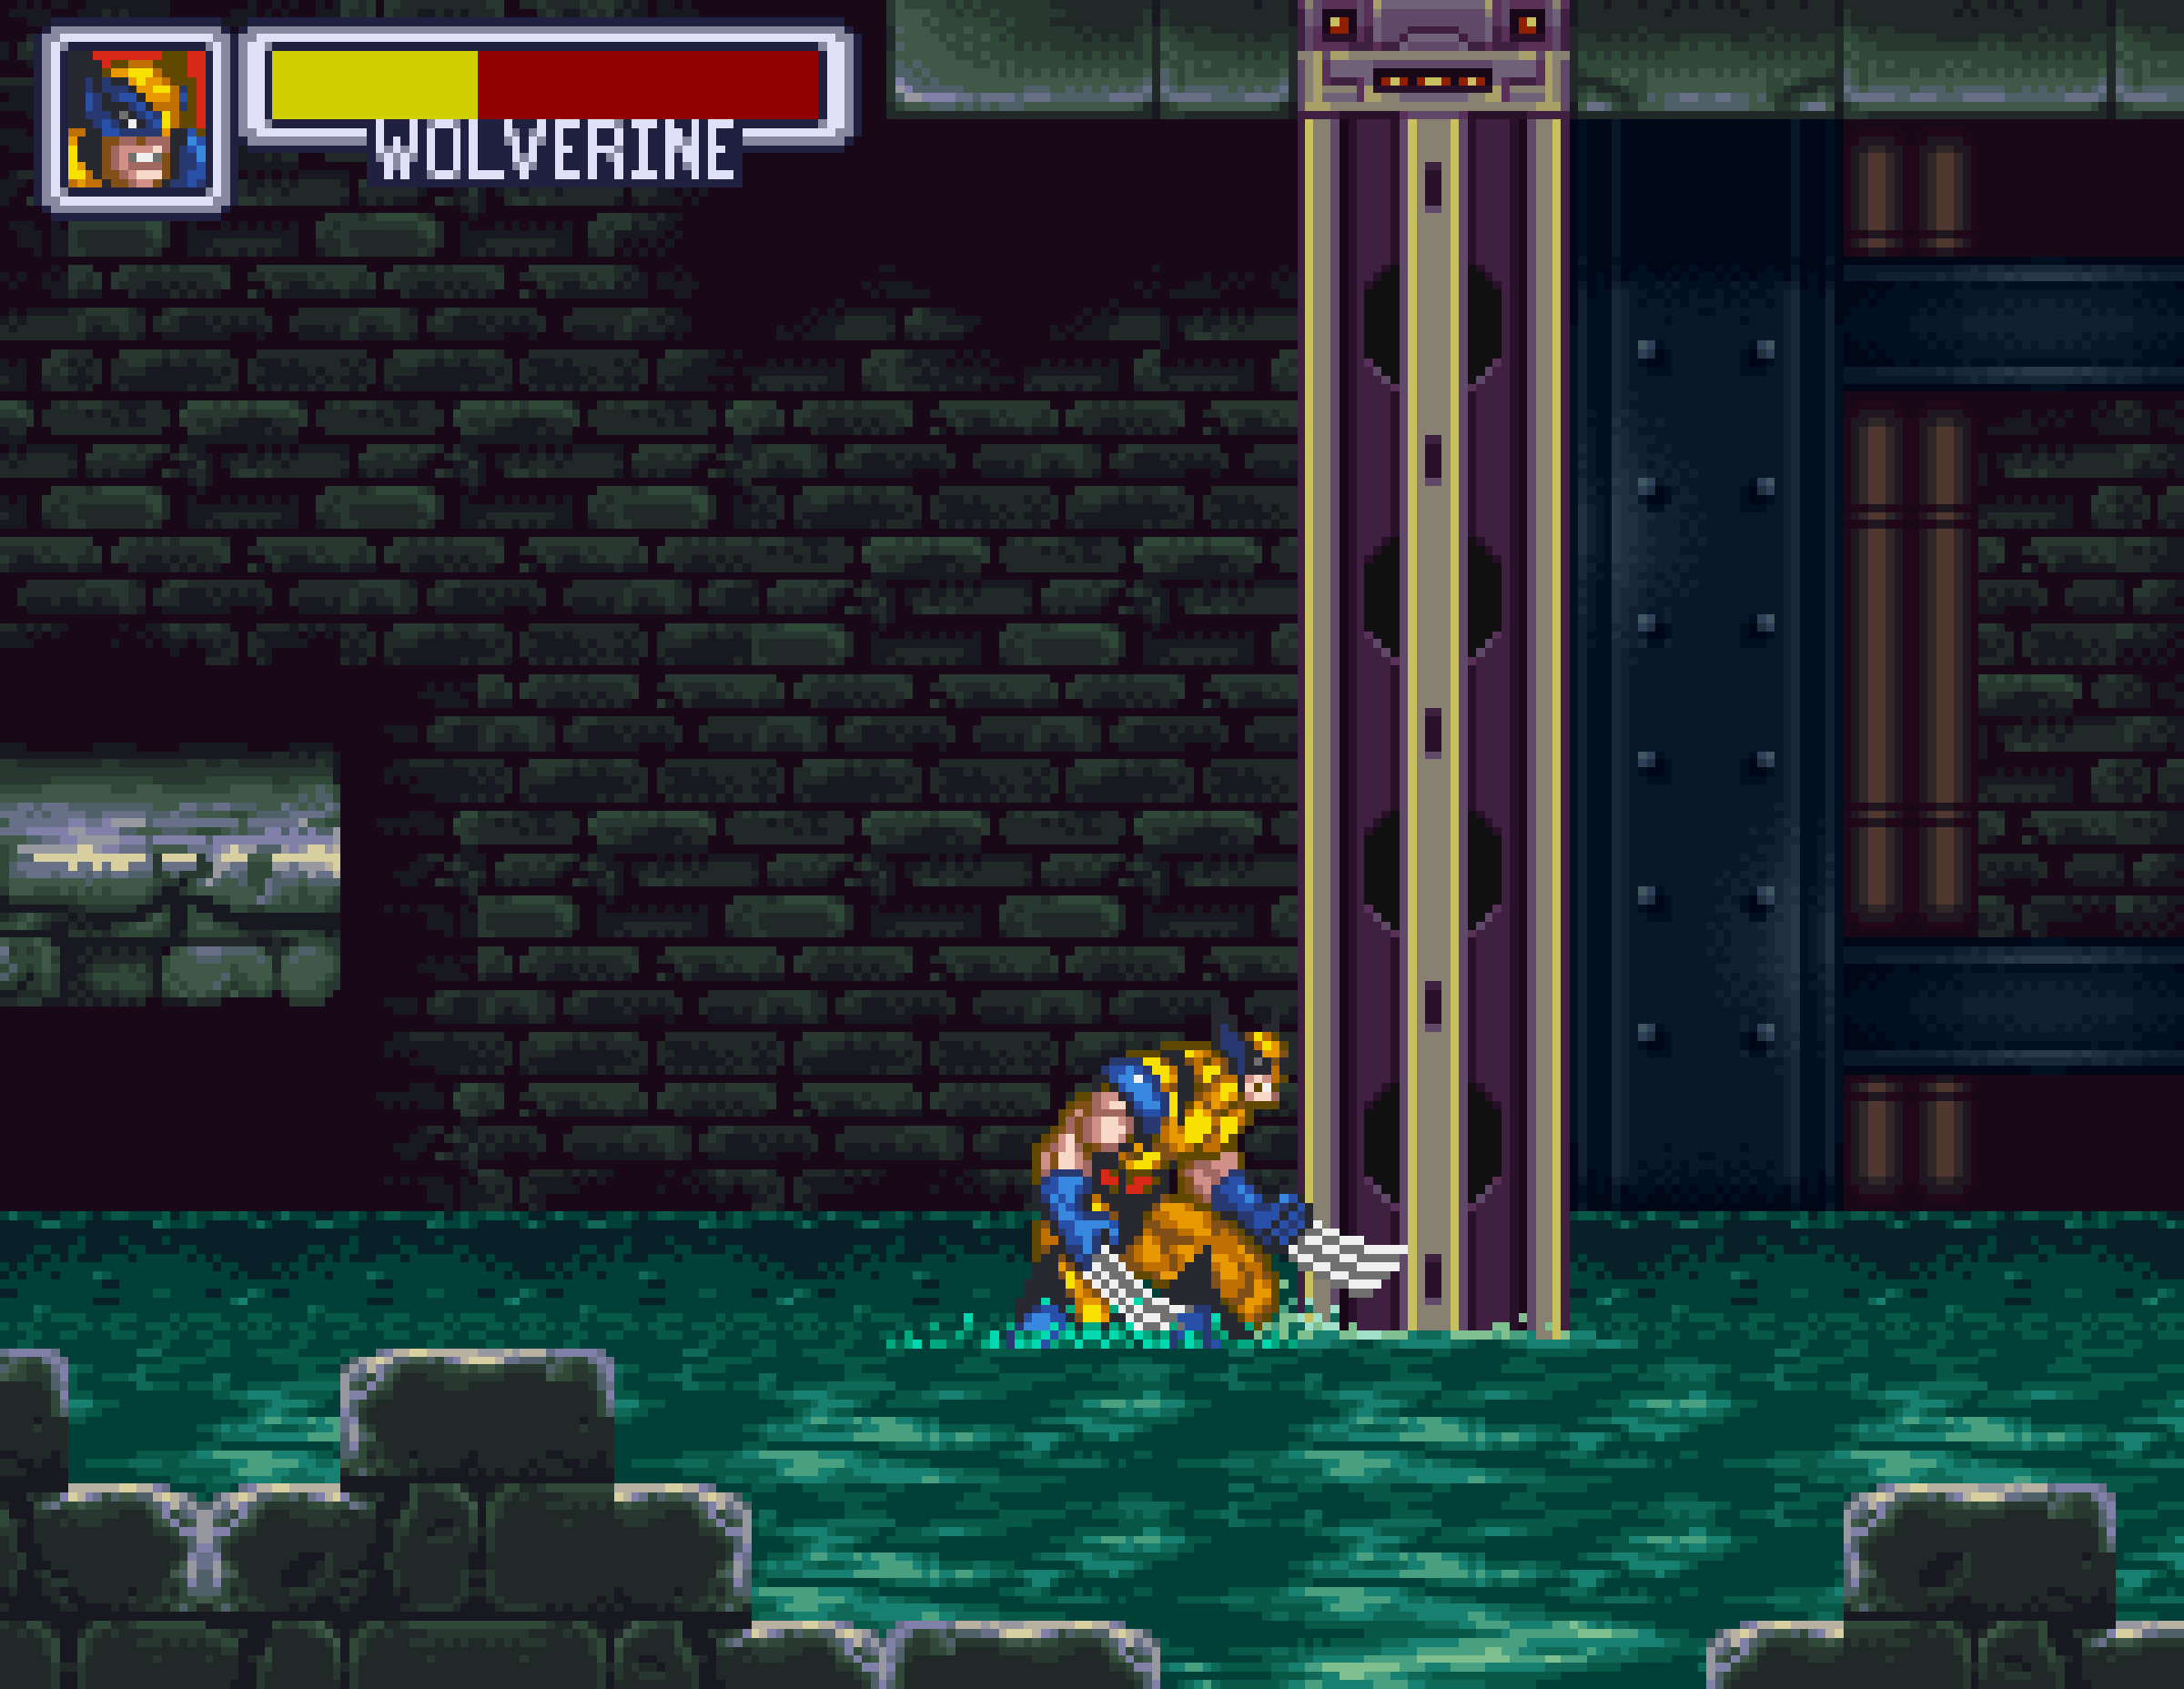
\includegraphics[width=0.49\textwidth]{fig-6a.png}
\hfill
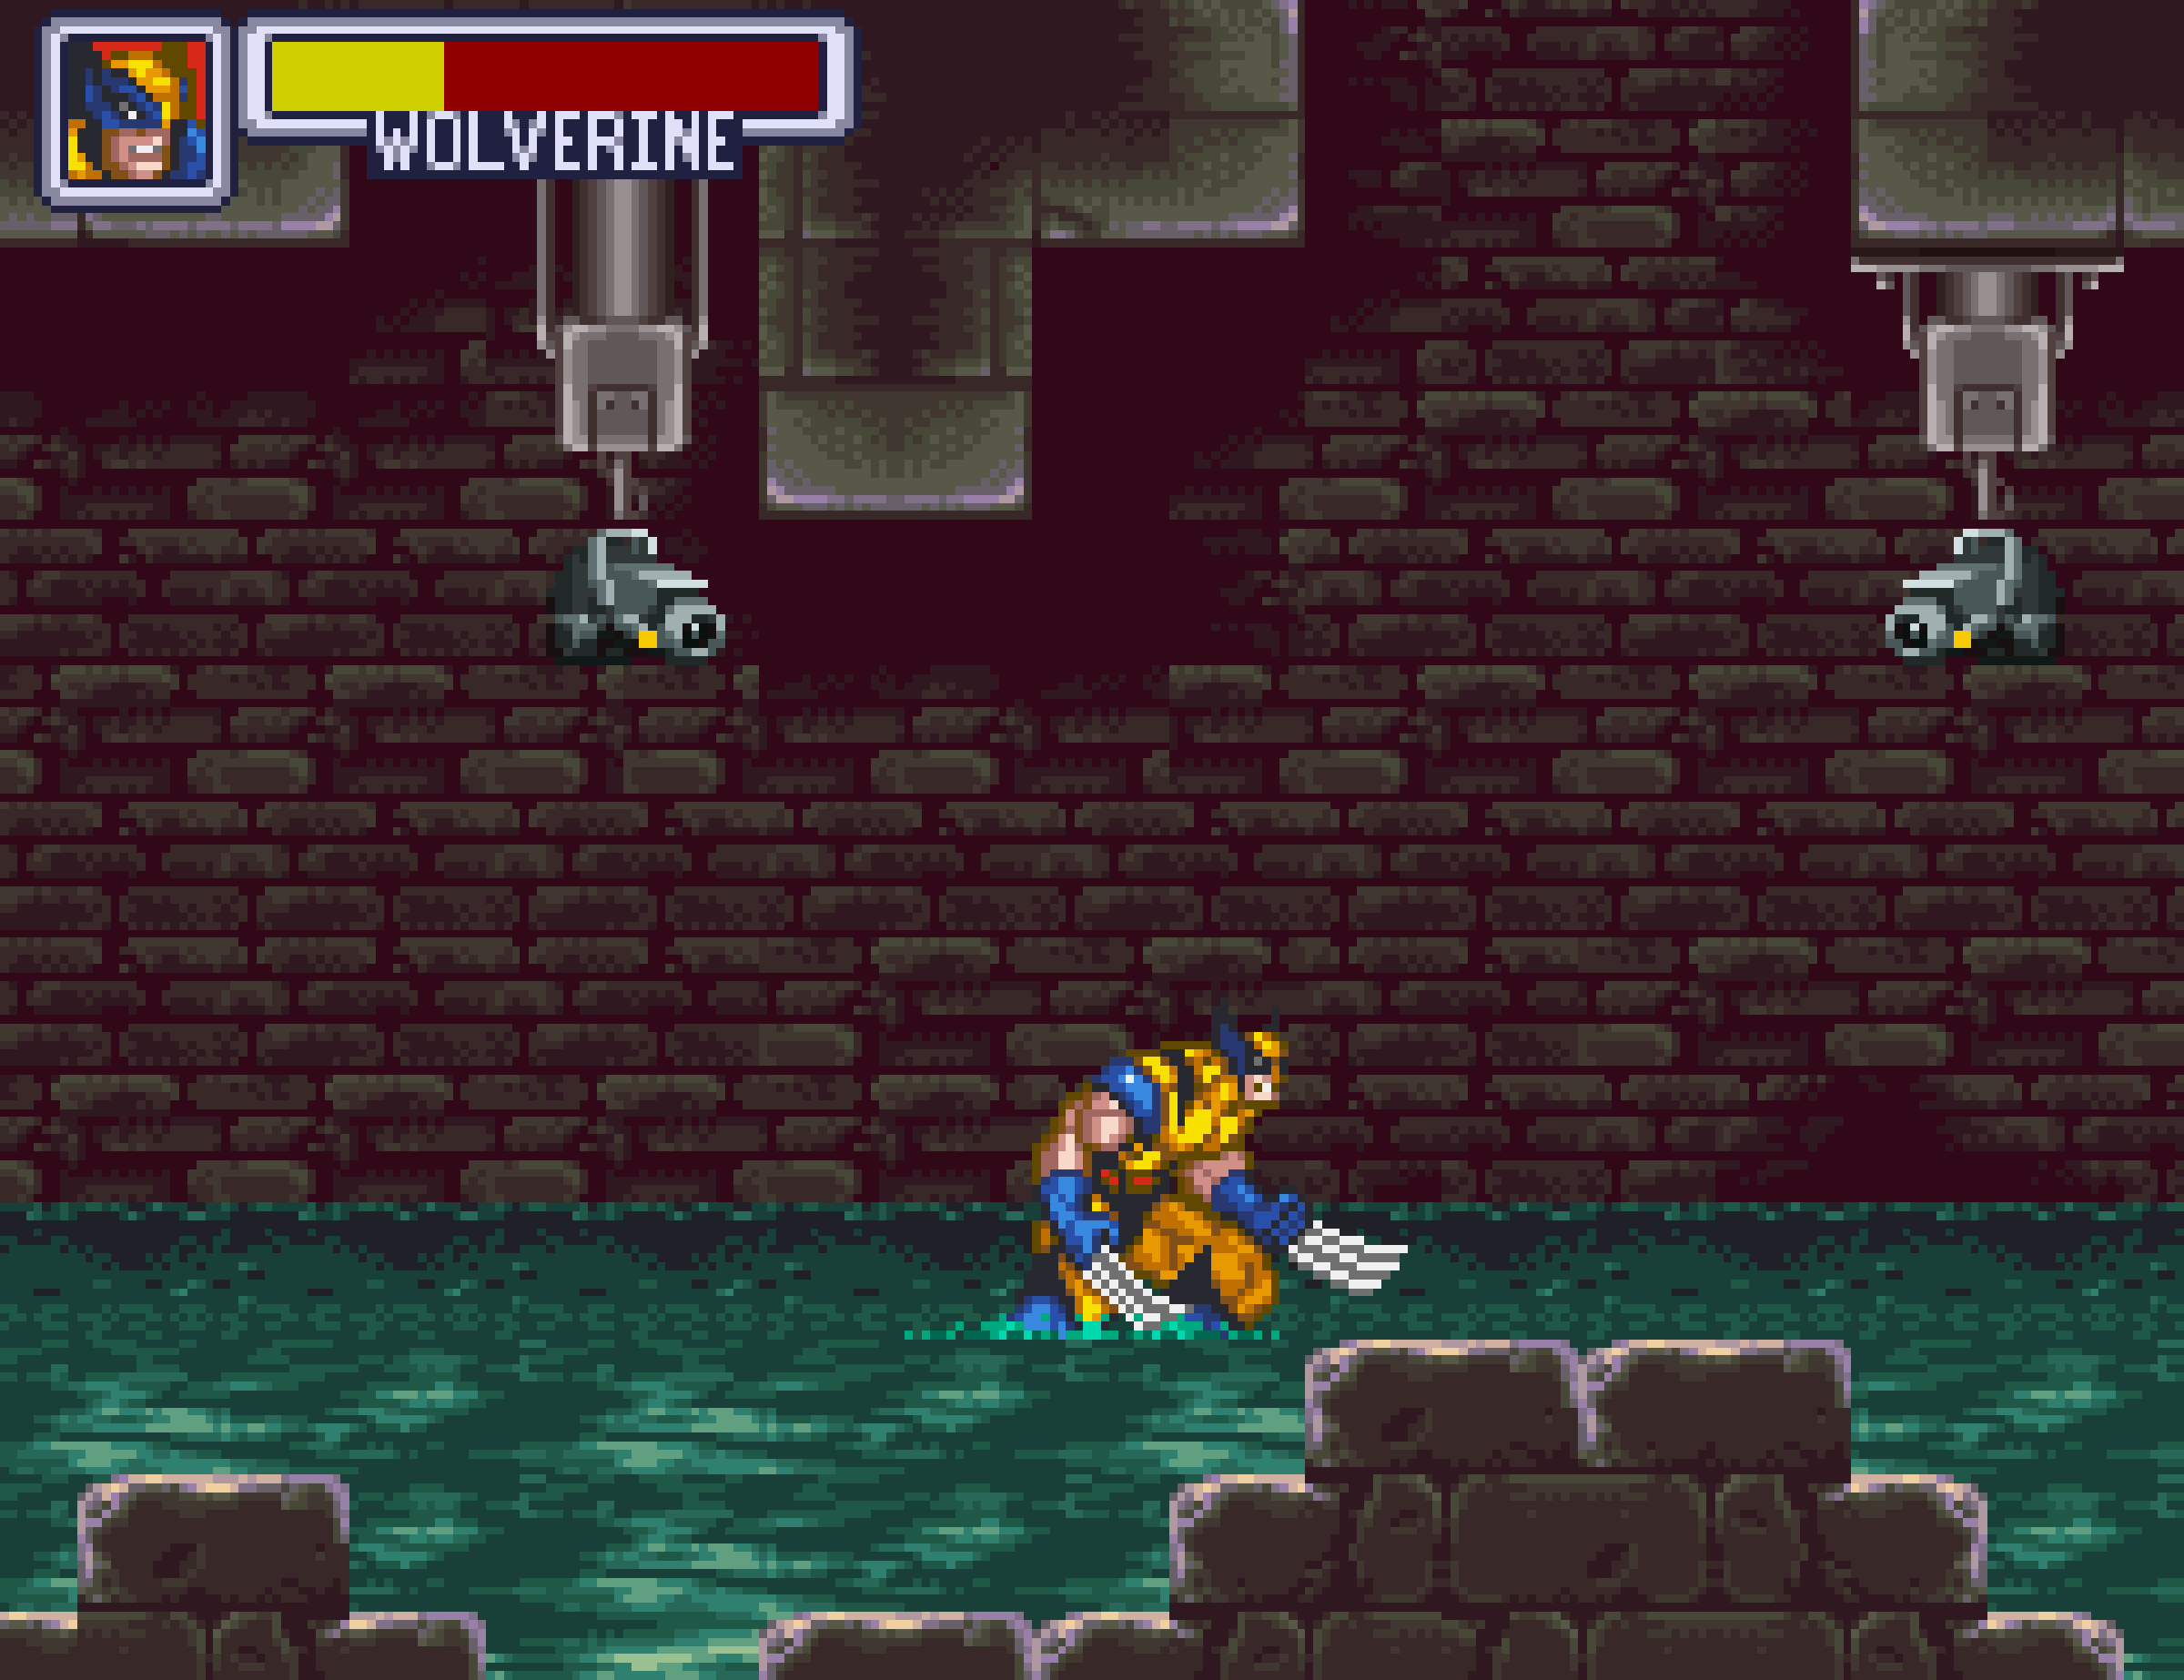
\includegraphics[width=0.49\textwidth]{fig-6b.png}
\caption{Tunnel.}
\label{fig-6ae6b}
\source{\textcite{capcom_marvel_1996}.}
\end{minipage}
\hfill
\begin{minipage}[t]{.47\textwidth}
\vspace{2pt}
\textbf{Canvas 3}, ‘Tunnel’: to get to this area, the player must destroy a metal barrier. The tunnel is protected by traps (spiked balls in chains) and security cameras. The cameras alert the enemies about the player's presence: an alarm sounds and a few enemies swarm in. The closed environment due to the low ceiling can be dangerous for the player, as they can be overwhelmed by the enemy forces.
\end{minipage}
\end{figure}


\begin{figure}[htbp]
\begin{minipage}[t]{.47\textwidth}
\vspace{0pt}
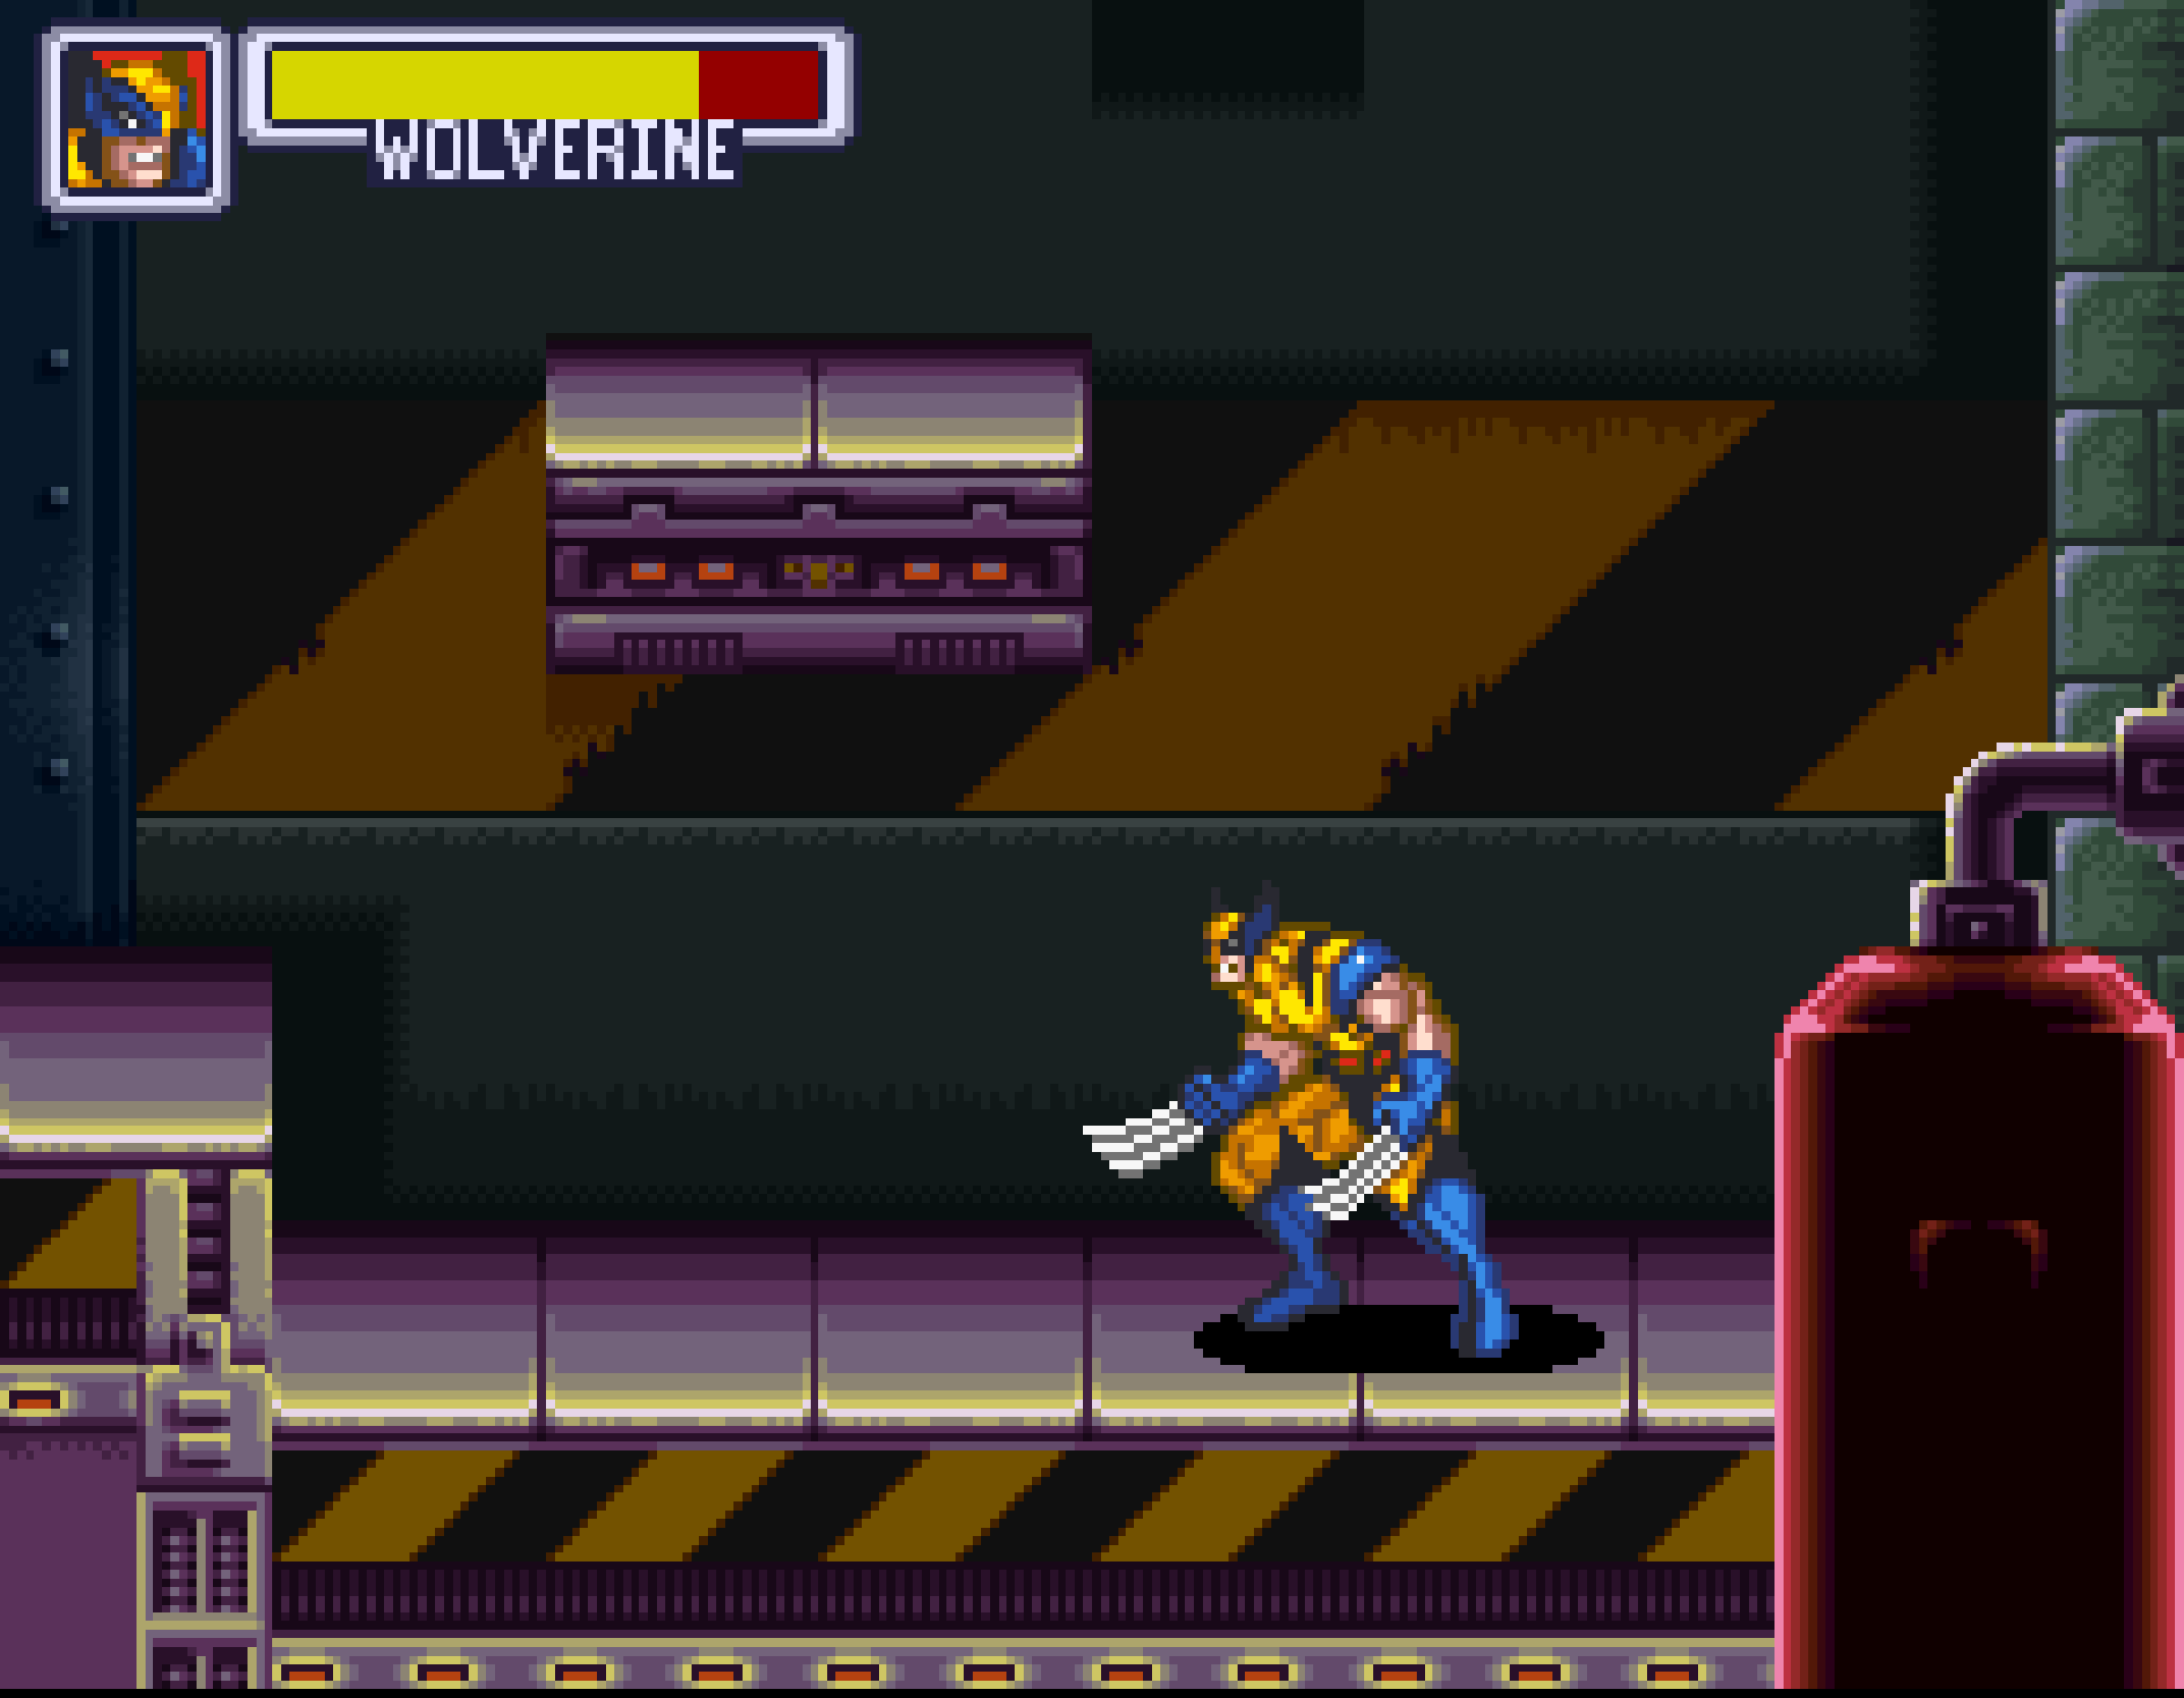
\includegraphics[width=\textwidth]{fig-7.png}
\caption{Lab.}
\label{fig-7}
\source{\textcite{capcom_marvel_1996}.}
\end{minipage}
\hfill
\begin{minipage}[t]{.47\textwidth}
\vspace{2pt}
\textbf{Canvas 4}, ‘Laboratory’: at the end of the tunnel, the player finds a purple laboratory. Unlike the previous three Canvases, the lab has laser cannons and futuristic-looking technology.
\end{minipage}
\end{figure}


\begin{figure}[htbp]
\begin{minipage}[t]{.47\textwidth}
\vspace{0pt}
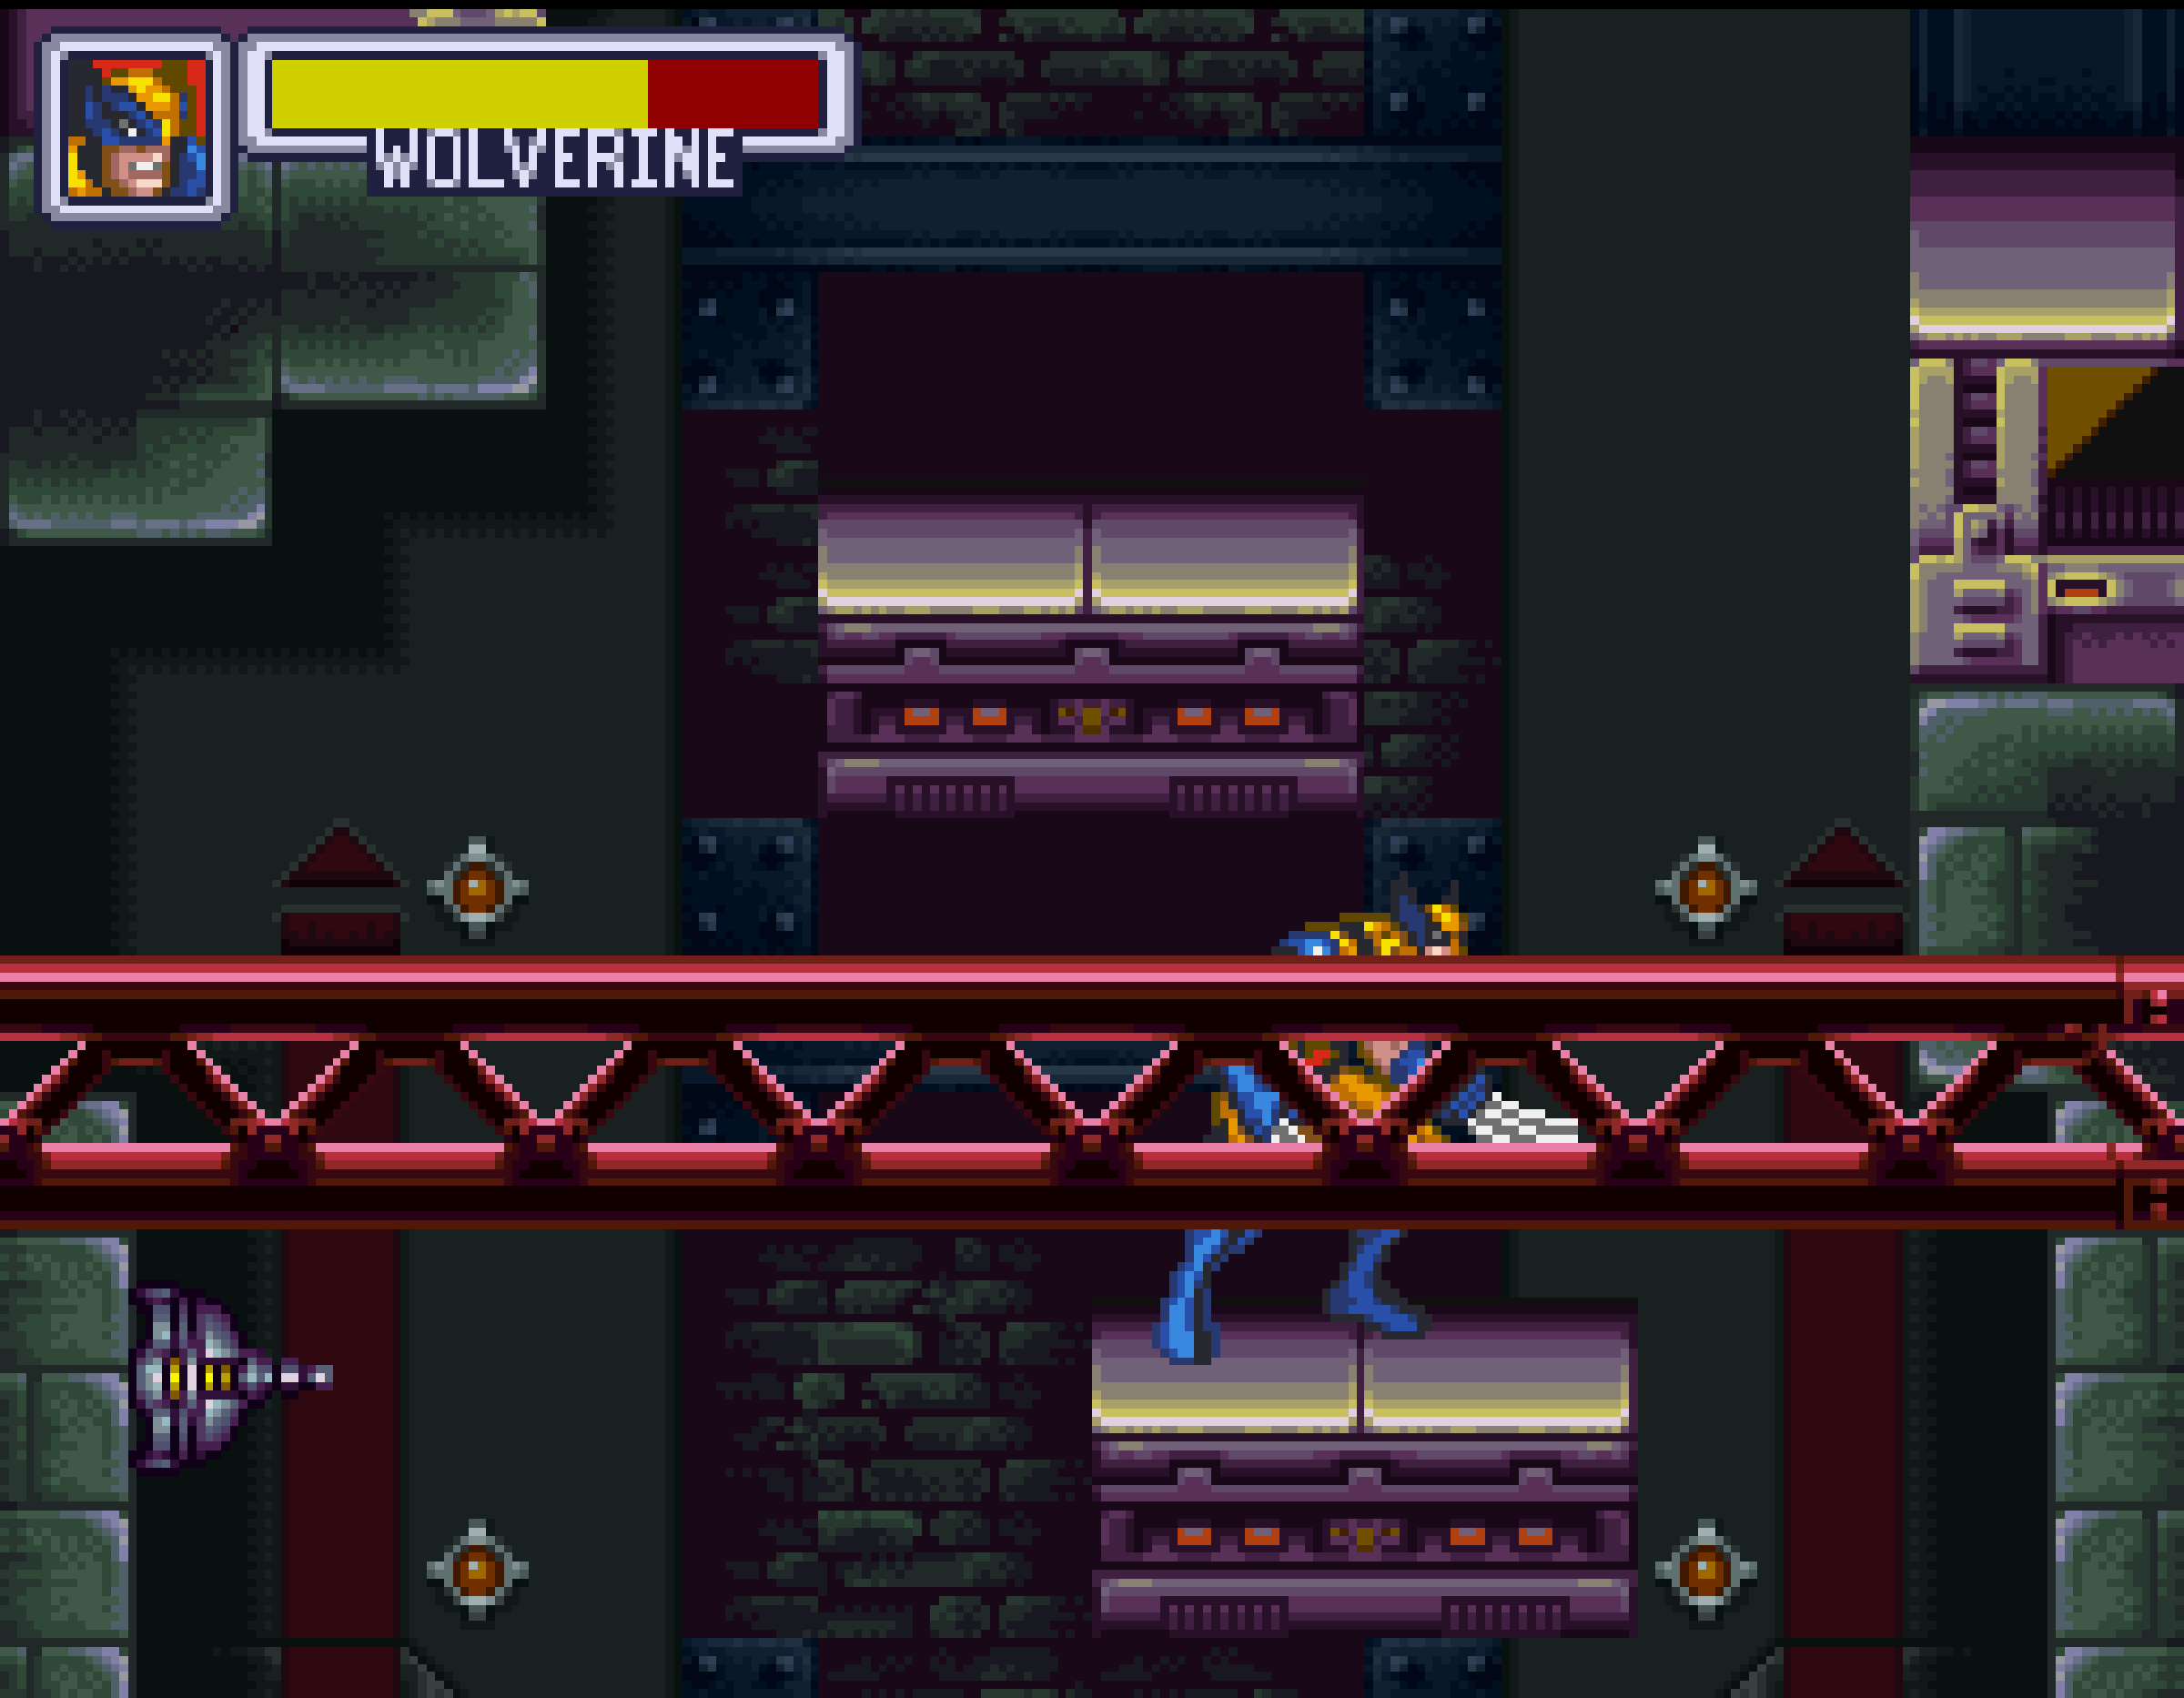
\includegraphics[width=\textwidth]{fig-8.png}
\caption{Lab.}
\label{fig-8}
\source{\textcite{capcom_marvel_1996}.}
\end{minipage}
\hfill
\begin{minipage}[t]{.47\textwidth}
\vspace{2pt}
\textbf{Canvas 5}, ‘Laboratory platforms’: the player must now climb the laboratory via purple platforms.
\end{minipage}
\end{figure}

\begin{figure}[htbp]
\begin{minipage}[t]{.47\textwidth}
\vspace{0pt}
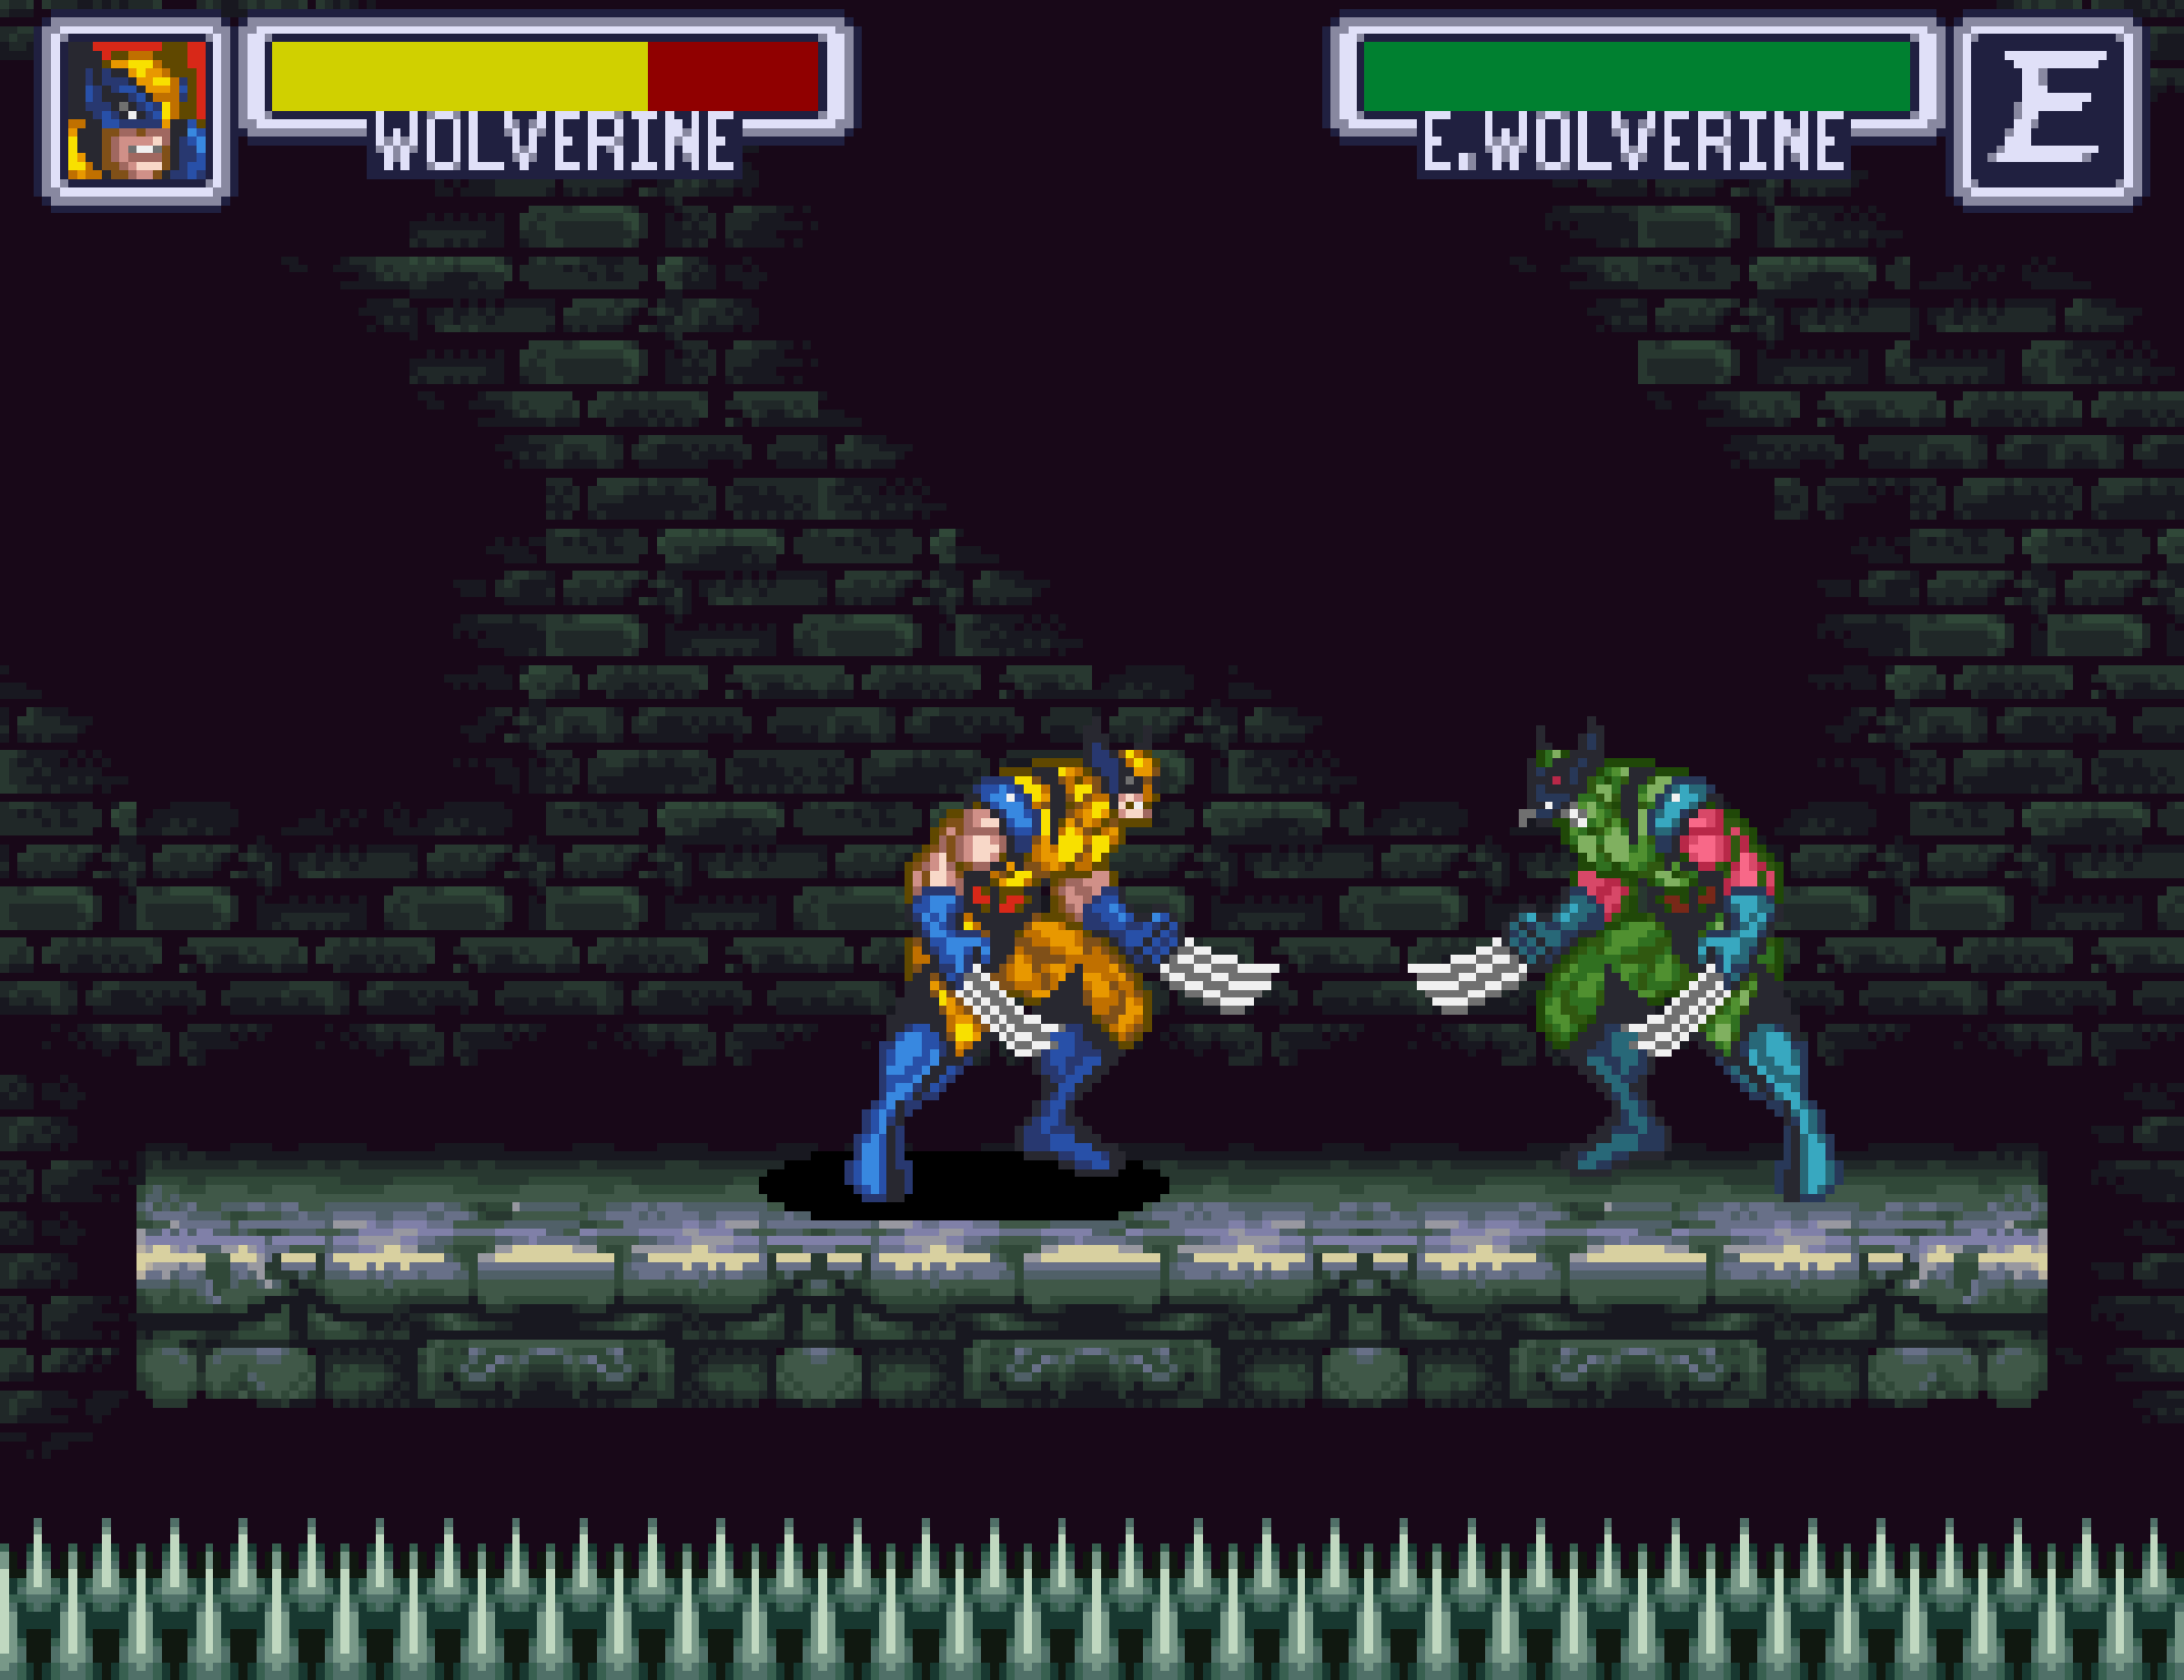
\includegraphics[width=\textwidth]{fig-9.png}
\caption{Boss room.}
\label{fig-9}
\source{\textcite{capcom_marvel_1996}.}
\end{minipage}
\hfill
\begin{minipage}[t]{.47\textwidth}
\vspace{2pt}
\textbf{Canvas 6}, ‘Boss room’: this is the last Canvas of the stage. The Amazon Forest theme is briefly interrupted and the Boss theme begins to play. The player must defeat the stage boss, a Wolverine clone.
\end{minipage}
\end{figure}


Through Linking analysis, we can correlate representational, i.e., interface (\textit{semiosis}) and interactive choices, i.e., level design (\textit{ludosis}) \textcite[p. 27]{egenfeldt-nielsen_understanding_2016}.

Furthermore, we can analyze how image and interaction are interwoven. The visual progression (forest [canvas 1] → ruins [canvas 2-3] → laboratory [canvas 4-6]) can correlate with the ludic interaction (variety in combat and increased difficulty), creating a dichotomy between 'primitive' and 'technological.' The stage is located in Brazil, which could lead to the interpretation that Brazil is characterized as a blend of nature and technology. However, the representation of these two halves is fundamentally different: the forest is depicted realistically (given the limitations of the Super Nintendo), while the laboratory is fictional and houses laser cannons, for example. Considering the presence of the enemies, it can be assumed that the technology in the ancient ruins is something they brought with them to defend the Infinity Gem. Thus, most of the technological elements on the stage are not naturally found in Brazil itself. These choices are closely related to other representations of Brazil, including other games by the developer Capcom (cf. \textcite{capcom_street_1991}, in which Brazil is represented as the Amazon Forest.

\subsubsection{Rhythm}\label{sec-idioma}
Rhythm "provides coherence and meaningful structure to events unfolding over time" \cite[p. 179]{van_leeuwen_introducing_2005} and is characterized by alternating between 'opposite poles,' two states \cite[p. 182]{van_leeuwen_introducing_2005}.

We propose that, apart from the sound mode, the game generates a 'flow' characterized by the alternation of ludic poles. This 'flow' is defined by the player's interaction with the game (the \textit{gameplay}) and by the game itself.

To analyze rhythm in the game, we highlight the beginning area of the stage. Enemy forces regularly stop the player. The alternation between movement and combat creates a multimodal rhythm in the game. Following \textcite[p. 187-8]{van_leeuwen_introducing_2005}, we suggest in \Cref{tbl01} that ludic rhythm has semiotic implications.

\begin{table}[htbp]
\begin{threeparttable}
\caption{Rhythm within \textit{Marvel Super Heroes in War of the Gems}.}
\label{tbl01}
\centering
\begin{tabular}{p{0.1\textwidth}p{0.2\textwidth}p{0.3\textwidth}p{0.3\textwidth}}
& Walk & Fight & Walk \\
\hline
Visual & River & River, platforms and enemies & River and traps \\
Interactive & Movement commands (walk and jump) & Movement commands (walk and jump) and combat commands & Movement commands (walk and jump) \\
Sound & Music & Music and sound effects & Music \\
\hline
\end{tabular}
\source{Created by the authors.}
\end{threeparttable}
\end{table}

In \Cref{tbl01}, we highlighted the semiotic changes depending on the ludic states (movement or combat). It is worth noting that the game does not synchronize the sound and interaction, but the music is interspersed with the sound effects of combat — punches, kicks, and special moves — to emphasize the different 'game positions' the player must take to progress through the stage.

\subsubsection{Composition}\label{sec-resumo}
Composition is a cohesive and structural principle for spatial modes. It organizes representative (i.e., ideational) and interactive (i.e., interpersonal) meanings through three interrelated systems: Informational Value, Salience, and Framing \cite[p.~179;198-217;274]{van_leeuwen_introducing_2005}.

\paragraph{Information value}\label{sec-secoes}
Information value refers to the positioning of elements, in the case of \textit{Marvel Super Heroes}, on the screen. Each 'zone' can imbue meanings to the participants positioned inside of it. The zones are as follows: left-right, top-bottom, and center-margins \cites[p. 179]{kress_reading_2020}. We show a screen of the game followed by the analysis of the zones in \Cref{fig010}.

\begin{figure}[htbp]
\centering
\begin{minipage}[t]{0.6\textwidth}
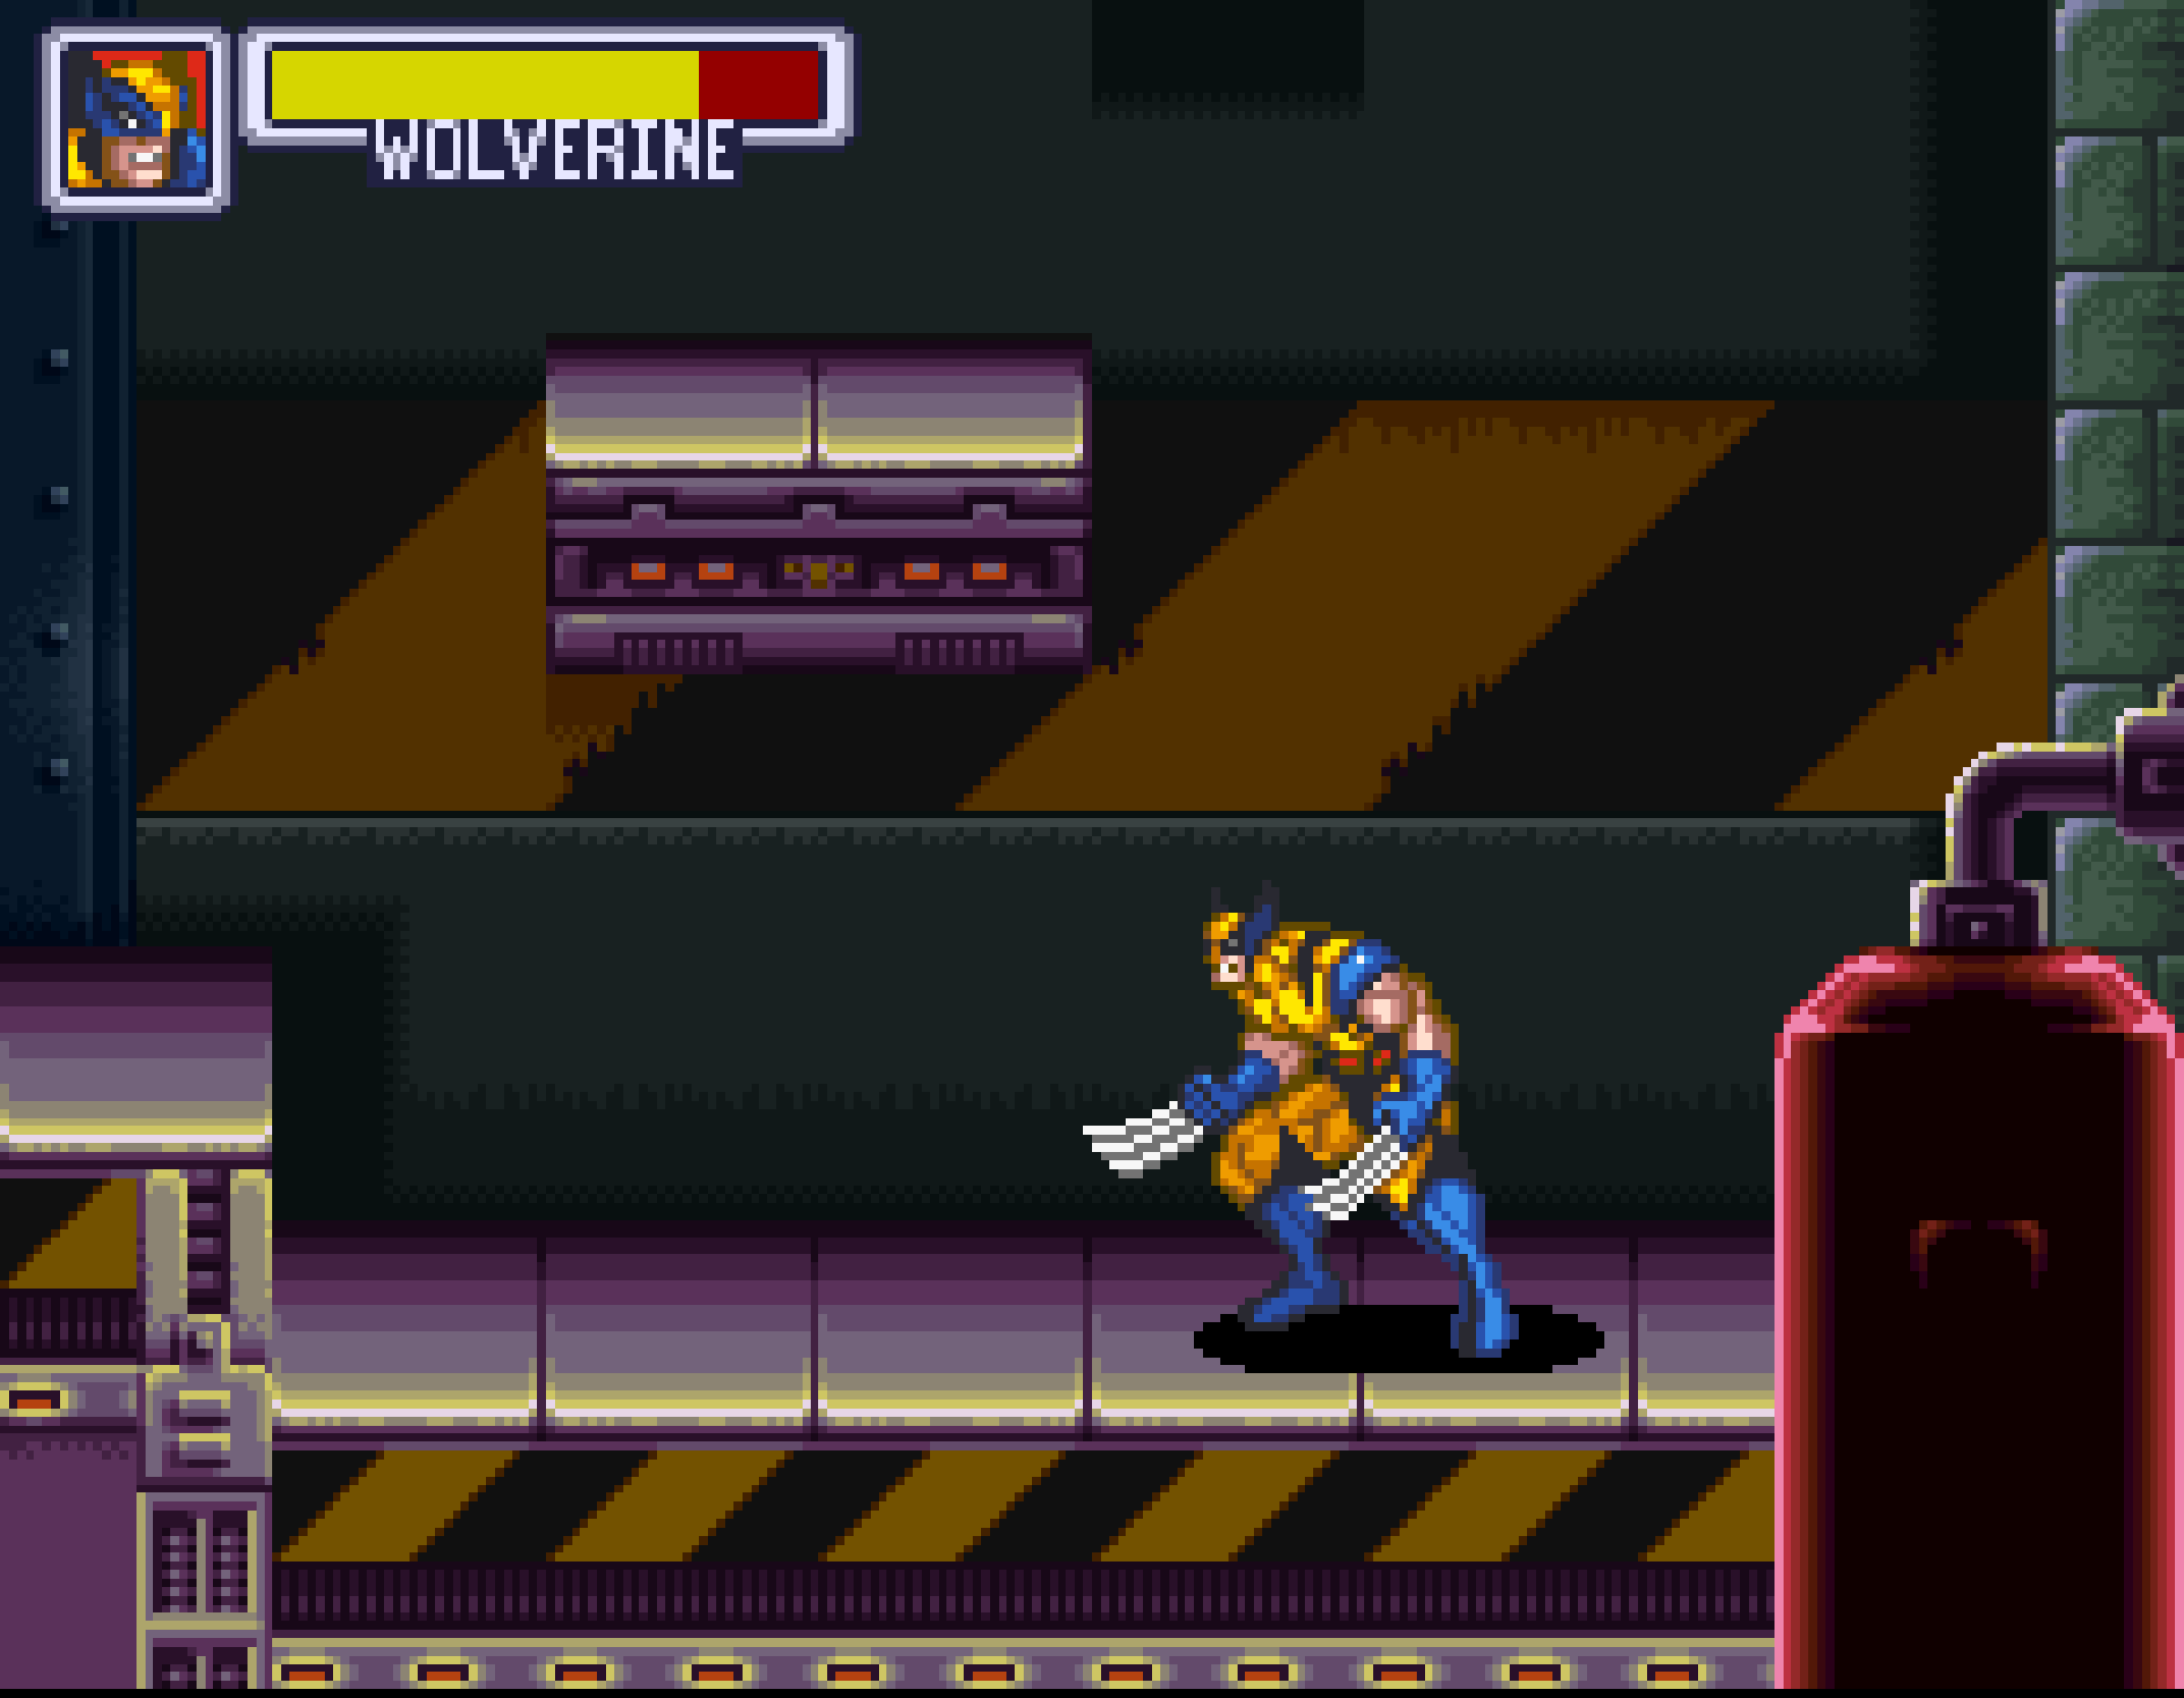
\includegraphics[width=\textwidth]{fig-010.png}
\caption{Wolverine at the stage’s opening screen.}
\label{fig010}
\source{\textcite{capcom_marvel_1996}.}
\end{minipage}
\begin{minipage}[t]{\textwidth}
\small
\begin{description}
    \item[Left-Right zones]: \textcite[p. 201-2]{van_leeuwen_introducing_2005} points out the semiotic potential of the left side signifying what is 'given,' while the right side signifies what is 'new.' This notion is significant in English writing, for example, as writing flows from left to right. In a two-dimensional game like \textit{Marvel Super Heroes} and many others, this connection also holds true: the stage goes from left to right, forming a continuum between what is known (given) and what is yet to come (new).

    \item[Top-Bottom zones]: the top-bottom dichotomy is filled with associative meaning. For example, the terms 'upper class,' 'ascending,' and 'heaven' imply that what is above is positive, while what is below — 'lower class,' 'descending,' 'hell' — is negative. \textcite[p. 204-5]{van_leeuwen_introducing_2005} suggests that what is above is usually represented as ideal (more abstract), while what is below is represented as real (less abstract). In \textit{Marvel Super Heroes}, as is common in 2D games, the HUD (heads-up display) appears at the top of the screen. In this case, the HUD consists of a simple life bar and the character's face and name. Since these are not diegetic elements, we can consider them more abstract, 'less real'.

    We hypothesize the following as to why this arrangement is commonly used: the game takes place on the ground; therefore, the creators dedicate the upper part of the screen as a 'non-playing area.' The player will rarely be in the upper area for long; thus the overlap between HUD and the player character is minimal, which would otherwise hinder the 'readability' of the game.

    \item[Center-margin zones]: similar to the top and bottom dichotomy, the center and margin also evoke associative meanings. Unlike the margins, the center is usually understood as an area of importance. According to \textcite[p. 198]{kress_reading_2020}, this distinction is also present in spatial modes: the participant placed in the center is often the most prominent; furthermore, the margins derive from the center. In \textit{Marvel Super Heroes}, as in many two-dimensional games, the camera is generally 'glued' to the player character, so that they are always in the center of the screen. Since the player character is the most important participant in the composition, there is an overlap between semiosis and interaction.
\end{description}
\end{minipage}
\end{figure}

\paragraph{Salience}\label{sec-format-simple}
Salience refers to the visual weight that a participant has, i.e., how much the referent is emphasized ('heavier') by visual choices. Some factors that affect the salience of a referent are relative size, detail, tonal contrast, positioning, and perspective \cites[p. 198]{van_leeuwen_introducing_2005}[p. 182]{kress_reading_2020}.

Returning to \Cref{fig010}, we propose that Wolverine is the most salient referent not only because he is the player character, but also because the creators employed several semiotic resources to enhance the character's "visibility" relative to the game world and its inhabitants (the enemies): he is more detailed than the enemies or the environment; the bright colors of his uniform stand out against the background; he is in the foreground; his relative size is larger than, for example, the pyramid in the background due to his positioning.

\paragraph{Framing}\label{sec-format-simple}
Framing refers to the disconnection of participants in the composition through frame lines, empty spaces, and disconnections. On the other hand, it can also convey connection by framing participants closely or in a comparable manner \cite[p.~277]{van_leeuwen_introducing_2005}. In summary, it establishes relationships of exclusion and belonging among participants in the composition \cite[p. 181-2]{kress_reading_2020}.

Video games are primarily framed by the screen, that is, by what is being displayed. Thus, some games consist of a single screen (e.g., Donkey Kong \cite{nintendo_donkey_1981}), while others present multiple screens in sequence. Within each of these frames, the game may also frame smaller elements. For example, the HUD and the 'playing area' are framed differently to convey that they are of different natures. In the case of \textit{Marvel Super Heroes}, the HUD is minimal, but it is still framed to separate it from the diegetic world by using thick white outlines.

\subsection{Composition and level design}\label{sec-outras-estr}
Composition can be applied to analyze the whole stage. In \textit{Marvel Super Heroes}, we can split the six Canvas into three groupings (\Cref{fig011}):

\begin{figure}[htbp]
 \centering
 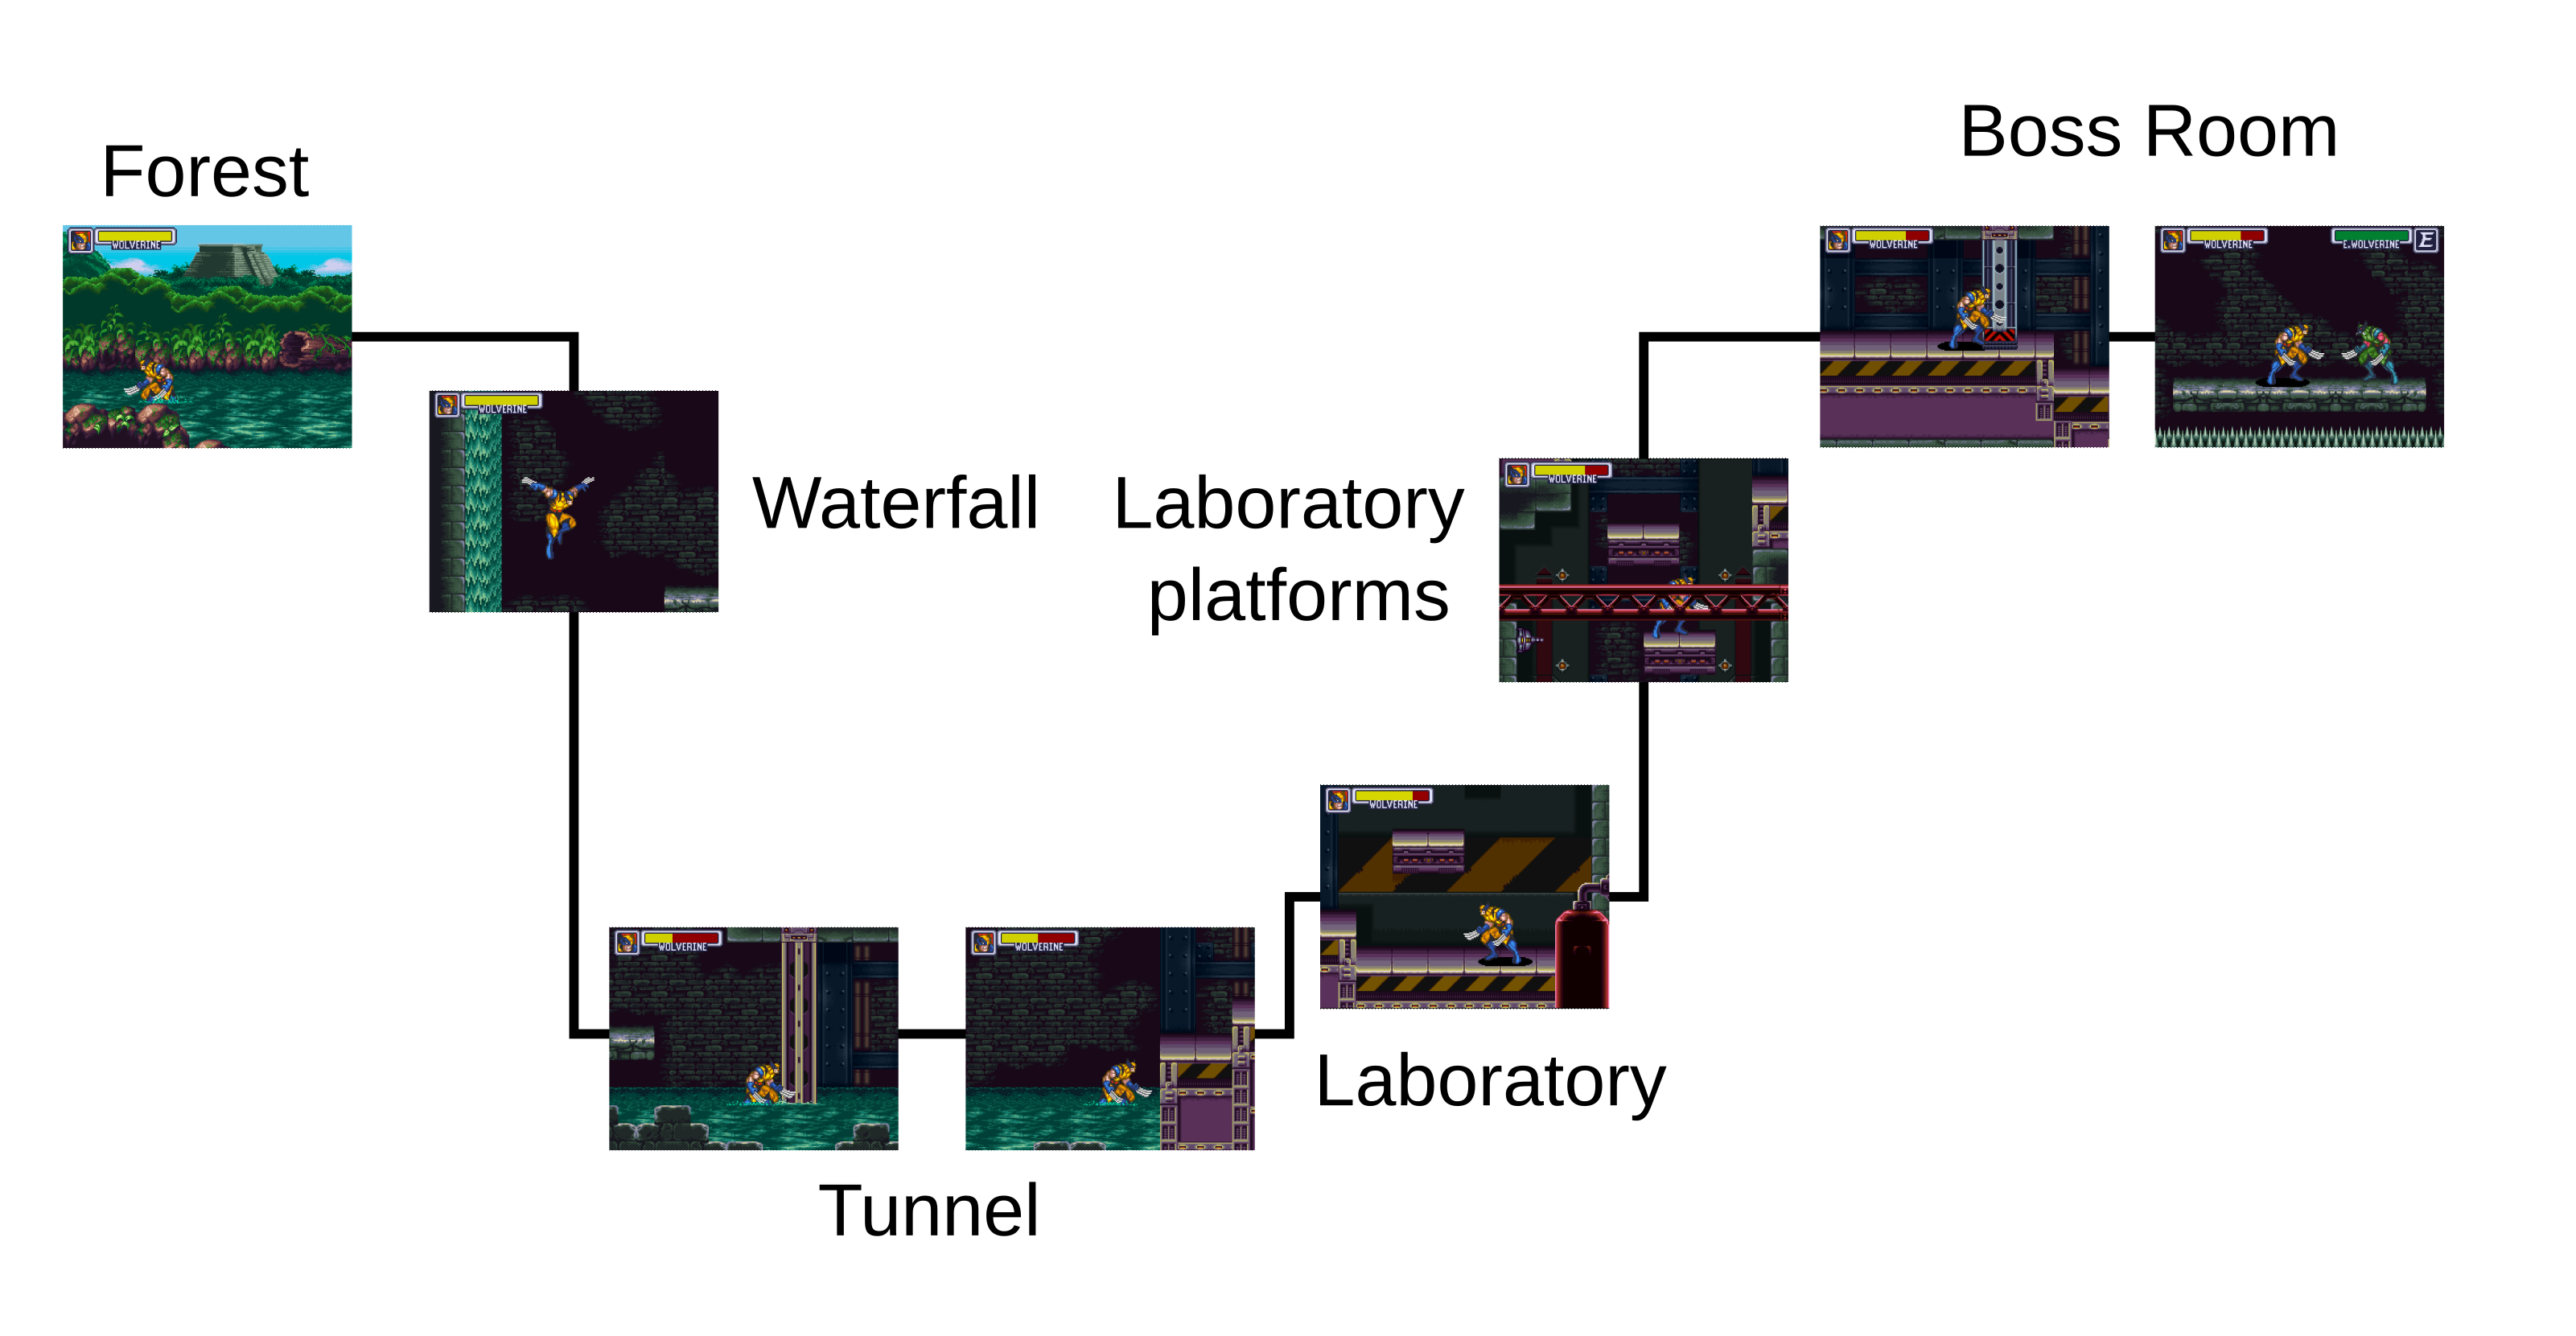
\includegraphics[width=\textwidth]{fig-011.png}
 \caption{Level design.}
 \label{fig011}
 \source{Screenshots from \cite{capcom_marvel_1996}; schema created by the authors.}
\end{figure}

Forest [Canvas 1]

Ruins [Canvas 2 and 3]

Laboratory [Canvas 4 to 6]

The boundaries (framing) between these three areas are different: the transition between the forest and the ruins is sudden, mediated by the Waterfall and the metal barrier, while the shift between the ruins and the laboratory is subtle: both spaces overlap. Based on \textcite[p.~13]{van_leeuwen_introducing_2005}, we propose that the forest is disconnected from the ruins, while the ruins intersect with the laboratory.

Regarding the represented participants, the ruins have no trees, but the water still flows, while in the laboratory neither trees nor water is present. Therefore, artificial participants supplant the natural ones. Visually, the hue conveys this gradual change: the stage goes from green and blue to green and then to purple. Finally, there are also the shapes of the participants: the forest is more irregular, while the laboratory features regular shapes. One meaning potential that arises from this choice is the association of irregularity with disorder and regularity with orderliness.

\section{Discursive analysis}\label{sec-listas}
Lastly, following \posscite[p.~110;p.~3-22;105~et~seq.]{van_leeuwen_introducing_2005,van_leeuwen_discourse_2008} discourse anatomy, we can discuss the choices employed by the creators in relation to the ideological and the intertextual dimensions of the chosen game. In \Cref{table02}, we present the description of the discursive categories and their application in \textit{Marvel Super Heroes}.

Transformations: transformations are the changes that a social practice or object undergoes when represented in a semiotic mode. We can express discourses as ‘social practice/event + ideas and attitudes about the chosen subject’ \cite[p. 94]{van_leeuwen_introducing_2005}.

\setlength\LTleft{-1in}\setlength\LTright{-1in}
\begin{small}
\renewcommand{\arraystretch}{1.5}
\begin{longtable}{
    >{\raggedright\arraybackslash}p{0.2\textwidth} 
    >{\raggedright\arraybackslash}p{0.92\textwidth}  
    }
\caption{Discursive analysis of the Amazonian stage.}
\label{table02}
\\
\toprule 
Transformation type & Description \\
\midrule
\multirow{4}{=}{Additive transformations} & 
\textbf{Participants}: relates to the addition of any participants to the represented object/social practice.
\begin{itemize}
    \item In \textit{Marvel Super Heroes}, the Mayan Pyramid is a participant added to the representation due to its perceived relatedness to the Amazon Forest. The implicit notion is that all American Peoples are 'the same' or the Amazon Forest is the space that encompasses all these different cultures.
\end{itemize} \\
& \textbf{Legitimation}: relates to the justifications to why something happens the way it happens, or should not happen, in the case of social practices. Regarding representations, legitimation presents the rationale behind the semiotic choices employed \cite[p. 20]{van_leeuwen_discourse_2008}. Next, we quickly summarize the legitimation types\footnote{\textcite{van_leeuwen_discourse_2008} proposes several systems of legitimation and purposes. Given the limitations of this article, we will not examine all the subsystems established by the author, only the main categories.}: 
\parfillskip=0pt \tabularnewline
&\begin{description}
    \item[Authorization]: based on tradition, recommendations, or laws, i. e., socially recognized authorities, personalized (e.g., specialists in an academic field) or not (e.g., laws) \cites[p. 105]{van_leeuwen_discourse_2008}.
    \item[Moral legitimation]: it “is based on values, rather than imposed by some kind of authority without further justification. In some cases, moral value is simply asserted by troublesome words such as 'good' and 'bad,' which freely travel among moral, aesthetic, and hedonistic domains and often combine with authority legitimation [...] but in most cases, moral evaluation is linked to specific discourses of moral value. However, these discourses are not made explicit and debatable. They are only hinted at, by means of adjectives such as 'healthy,' 'normal,' 'natural,' 'useful,' and so on” \cites[p. 109-110]{van_leeuwen_discourse_2008}.
    \item[Rationalization]: “legitimation by reference to the goals and uses of institutionalized social action and to the knowledge that society has constructed to endow them with cognitive validity” \cites[p. 106]{van_leeuwen_discourse_2008}.
    \item[Mythopoesis]: “legitimation conveyed through narratives whose outcomes reward legitimate actions and punish nonlegitimate actions” \cites[p. 106]{van_leeuwen_discourse_2008}.
\end{description}
\parfillskip=0pt \tabularnewline
&\begin{itemize}
    \item The main legitimation strategy deployed in \textit{Marvel Super Heroes} is Authorization: the game uses several images (and, therefore, discourses) conventionally associated with Brazil, be it the Amazon Forest or the Mesoamerican iconography. That is, legitimation arises from a tradition \cites[p. 108]{van_leeuwen_discourse_2008} of representations in other media: movies, for example, such as \textit{Creature from the Black Lagoon} (Universal Studios, 1954), in which researchers encounter a monster in the Amazon Forest.
\end{itemize}
\\
 & 
\textbf{Evaluation}: evaluations can pertain to the whole practice/object or to parts of it \cites[p. 21]{van_leeuwen_discourse_2008}. They are not legitimations since they can appear in a text without being legitimized. However, they are related to a legitimate discourse, such as the religious discourse, which dictates what is morally good or bad \cites[p. 21]{van_leeuwen_discourse_2008}.

\begin{itemize}
    \item It is possible to propose that the game evaluates the Amazonian region (and Brazil through metonymy) as lesser in comparison to the other countries under a discourse that values technology and progress. The forest 'covers' the laboratory, the only construction aside from the Pyramid, an ancient structure. Likewise, the game 'hides' Brazil under the blanket representation of the Amazon Forest.
\end{itemize}
\\
& \textbf{Purposes}: relates to the purpose of the practice or object’s representation \cites[p. 21]{van_leeuwen_discourse_2008}. Below, we summarize the necessary elements for the discursive construction of the purposeful action \cites[p. 126]{van_leeuwen_discourse_2008}: 
\begin{description}
    \item[Purposeful action]: that is, the action whose purpose is to be constructed
    \item[Purpose]: itself a process, an action, or a state
    \item[Purpose link]: the relation of purposefulness between these two.
\end{description}
\begin{itemize}
    \item The representation of Brazil in the game attends firstly to create a stage based on the Amazon Forest, which leads to representational and interactive purposes. Broadly, we propose that the Amazonian stage serves the purpose of creating a 'forest area,' so common in older games, just like 'desert' and 'lava' areas.
\end{itemize}
\\
\midrule
Non-Additive transformations & 
\textbf{Substitutions}: the transformation of practices/objects into semiotic elements is crucial for the meaning-making processes \cites[p. 17]{van_leeuwen_discourse_2008}. Aside from that, usually substitutions involve the transformation of concrete referents into abstract ideas or vice versa \cites[p. 111]{van_leeuwen_introducing_2005}.
\begin{itemize}
    \item Brazil, a political unit (abstract), is materialized under the guise of the Amazon Forest (concrete) in the game. At the same time, the forest (concrete) becomes a connotator of ‘primitiveness,’ (abstract), which applies to Brazil as a whole.
\end{itemize}
\\
 & \textbf{Exclusion (or deletion)}: involves the exclusion of a participant that composes the social practice/object represented semiotically \cites[p. 110]{van_leeuwen_introducing_2005}[p. 18]{van_leeuwen_discourse_2008}. Two major types of exclusion are suppression, when there are no references to the deleted element \cite[p. 29]{van_leeuwen_discourse_2008}, and backgrounding, when the deletion occurs only partly and we can still infer the missing participant, although not entirely \cite[p. 29]{van_leeuwen_discourse_2008}.

 \begin{itemize}
     \item The game suppresses the urban areas of Brazil, which can lead to an image of the country solely as a forest.
 \end{itemize} 
 \\
 & \textbf{Rearrangement}: the participants from the social practice/object can be represented in an order different from the original, staged order \cites[p. 110]{van_leeuwen_introducing_2005}[p. 18]{van_leeuwen_discourse_2008}.

 \begin{itemize}
     \item Given the interactive nature of games, most often the action will be linear and dependent on the player’s command. In more complex/narrative-driven games, the creators can employ, for instance, \textit{flashbacks}, that can break this flow of action.
 \end{itemize}
\\    
\bottomrule
\source{Created by the authors.}
\end{longtable}
\end{small}

\section{Conclusions}\label{sec-figuras-tabelas}
The toolkit presented here enables the visual analysis of video games, considering both their interactive and multimodal nature. Thus, visual analysis can be enhanced by taking into account the interface between images, other semiotic modes, and ludic interaction in the meaning-making processes. This is also true for analyzing other modes, such as the verbal and sound modes, which, although not the focus of this paper, are fundamental to convey meaning and information to players.

This multifaceted approach tailored specifically for video games stretches itself to the discursive dimension, an aspect worth noting since games were considered mere 'toys' for decades. In a relatively simple game such as \textit{Marvel Super Heroes}, we were able to discuss how the creators’ semiotic choices correlated both with discourses about Brazil and with the 1990s sociocultural context, especially to the environmental discussions at the time, which were the probable defining factor for the construction of the Amazon Forest as a metonymy for Brazil.

Thus, we can track down a direct correlation between semiosis and discourses because games, as texts, are potential (re)producers of ideologically instantiated signs. In \textit{Marvel Super Heroes}, the game is not the only one to associate Mesoamerican iconography with the Amazon Forest, but, simultaneously, it reproduces these referents and serves as a potential source for iconographic reproduction. In modern games, the representational and discursive capacity is even more refined, which demands further theorization to analyze the meaning-making processes, the conveyed discourses and stereotypes, and how the employed semiotic resources are instrumental in these processes particularly due to their interactive nature, which singularizes them from other mediums.


\section{Acknowledgments}\label{sec-quotesandfootnotes}
The research for this paper was supported by FAPESP (Fundação de Amparo à Pesquisa do Estado de São Paulo), grant 20/13090-1.

\printbibliography\label{sec-bib}
% if the text is not in Portuguese, it might be necessary to use the code below instead to print the correct ABNT abbreviations [s.n.], [s.l.]
%\begin{portuguese}
%\printbibliography[title={Bibliography}]
%\end{portuguese}


%full list: conceptualization,datacuration,formalanalysis,funding,investigation,methodology,projadm,resources,software,supervision,validation,visualization,writing,review
\begin{contributors}[sec-contributors]
\authorcontribution{André de Oliveira Matumoto}[conceptualization,formalanalysis,resources,investigation,methodology,visualization,writing]
\authorcontribution{Paulo Roberto Gonçalves-Segundo}[conceptualization,resources,validation,review]
\end{contributors}


\end{document}

